% ============================================================
%  GamefyDB — PFE Report  |  Chapters 4, 5 & 6 + Conclusion
%  Append this content inside the main document, before \end{document}
% ============================================================

% Placeholder macro for figures still to be captured.
% Already defined in rapport_chapters1_2.tex; \providecommand makes this
% file safe to compile both standalone and as an included part.
\providecommand{\todoFigure}[2][0.7\textwidth]{%
  \fcolorbox{red!60!black}{red!5}{%
    \parbox{#1}{\centering\vspace{0.6cm}%
      \textcolor{red!60!black}{\textbf{[TODO --- insert figure]}}\\[4pt]
      \textit{#2}\vspace{0.6cm}}}%
}

% ============================================================
%  CHAPTER 4
% ============================================================
\chapter{Sprint 2: Star Schema and Data Export}

\section{Introduction}

Sprint~2 builds on the clean DataFrames produced in Sprint~1. Its scope covers user
stories US-05 through US-07: constructing the four dimension tables and the two fact
tables that make up the GamefyDB star schema, then writing everything to disk in the
format Power~BI expects. By the end of the sprint, the pipeline is end-to-end: raw
Excel files go in, a ready-to-load star schema comes out.

\section{Sprint 2 Goals}

The goals agreed with the Product Owner for this sprint were the following.
They follow naturally from the dimensional model defined in Sprint~0 and from
the data quality work completed in Sprint~1.

\begin{itemize}
  \item \textbf{Dimension tables with surrogate keys.} Four dimensions
        (\textit{dim\_cashier}, \textit{dim\_terminal}, \textit{dim\_item},
        \textit{dim\_member}), each one keyed by a sequential integer
        starting at~1 so the fact tables can reference them through compact
        foreign keys.
  \item \textbf{Two fact tables with verified referential integrity.}
        \textit{fact\_transaction} for the cash register events and
        \textit{fact\_session} for the gaming sessions, both with their
        foreign keys resolving cleanly against the corresponding dimensions.
  \item \textbf{Power-BI-ready CSV output.} The six tables must be exported
        as UTF-8-BOM CSV files under \texttt{output/powerbi\_star/} so that
        Power~BI and Excel both render French characters and Arabic
        transliterations correctly without manual locale tweaks.
  \item \textbf{One-shot reproducibility.} A single \texttt{python run.py}
        command must read the four source files and emit the complete star
        schema, with no intermediate manual step.
\end{itemize}

\section{Sprint 2 Backlog}

Table~\ref{tab:sprint2_backlog} lists the tasks committed to this sprint.

\begin{longtable}{>{\bfseries}p{1.3cm} p{4.2cm} p{7cm}}
  \caption{Sprint 2 Backlog.\label{tab:sprint2_backlog}} \\
  \toprule
  \textbf{ID} & \textbf{User Story} & \textbf{Tasks} \\
  \midrule
  \endfirsthead
  \toprule
  \textbf{ID} & \textbf{User Story} & \textbf{Tasks} \\
  \midrule
  \endhead
  \bottomrule
  \endfoot

  US-05 & As an analyst, I want four normalised dimension tables with surrogate keys.
        & Build \textit{dim\_cashier}, \textit{dim\_terminal}, \textit{dim\_item},
          and \textit{dim\_member} from the cleaned DataFrames; assign sequential
          integer primary keys. \\[4pt]

  US-06 & As an analyst, I want two fact tables with foreign-key references to the
          dimensions.
        & Build \textit{fact\_transaction} from the cash data and
          \textit{fact\_session} from the sessions data; resolve FK references to
          all four dimension tables. \\[4pt]

  US-07 & As an analyst, I want to export the full star schema as CSV files ready
          for Power~BI.
        & Implement the export step in \texttt{run.py}; write each table to
          \texttt{output/powerbi\_star/} with UTF-8-BOM encoding so Power~BI
          reads French characters correctly. \\
\end{longtable}

\section{Design Refinement}

During Sprint~0, the product backlog described eight output tables — four dimensions
and four fact tables. After inspecting the actual source data more carefully during
Sprint~1, the design was refined:

\begin{itemize}
  \item \textbf{Stock movements} were absorbed into \textit{dim\_item}. All stock
        records in the source file are outgoing sales — there are no restock entries.
        Because there is only one direction of movement, a dedicated fact table adds
        no analytical value; instead, quantity sold and total revenue are aggregated
        directly into the item dimension.

  \item \textbf{Member statistics} were kept as \textit{dim\_member}. The members
        file contains one summary row per member — cumulative totals, not individual
        events — so it naturally fits a dimension rather than a fact table.
\end{itemize}

The final schema therefore has six tables: four dimensions and two facts. This
simplification makes the Power~BI data model easier to navigate without losing any
of the required KPIs.

\section{Implementation of the Transformer Stage}

\subsection{Building the Dimension Tables}

\subsubsection{dim\_cashier}

The cashier dimension is built by collecting all distinct cashier names across the
three transactional domains — cash, sessions, and stock — sorting them alphabetically,
and assigning a sequential surrogate key starting at~1. The five cashier accounts
in the source data (\textit{guds}, \textit{monta}, \textit{taktek},
\textit{yassine}, \textit{youssef}) all appear in the result.

\subsubsection{dim\_terminal}

The terminal dimension is derived exclusively from the sessions file, since that is
the only source that records terminal names reliably. Each unique \texttt{(terminal,
terminal\_type)} pair becomes one row. The \texttt{terminal\_type} column is computed
during cleaning: terminals whose names contain \texttt{PS5} become \textit{PlayStation},
those containing \texttt{VIP} become \textit{VIP PC}, and all others become
\textit{Standard PC}. The final dimension contains 16 terminals.

\subsubsection{dim\_item}

The item dimension aggregates the stock table by item name, retaining the first
observed category, the median unit price, total quantity sold, and total revenue.
Median is used instead of mean for the unit price so that occasional data-entry errors
do not distort the representative price. The dimension contains 17 distinct items.

\subsubsection{dim\_member}

The member dimension is a direct copy of the cleaned members DataFrame with no
further aggregation. It contains 66 unique members, each described by their username,
first name, last name, cumulative session duration in minutes, and cumulative spend
in TND across usage, orders, USB data, and total.

\subsection{Building the Fact Tables}

\subsubsection{fact\_transaction}

The transaction fact table is built from the cash DataFrame. Each row represents one
cash register event — an income or expense entry recorded by a cashier. The foreign
key resolution works as follows:

\begin{itemize}[noitemsep]
  \item \textbf{cashier\_id} — looked up from the cashier name map built from
        \textit{dim\_cashier}.
  \item \textbf{terminal\_id} — assigned only for \textit{Computer Incomes} and
        \textit{Playstation Incomes} categories, since those are the only transaction
        types tied to a terminal. Rows in other categories carry a null terminal
        reference.
  \item \textbf{item\_id} — assigned only for \textit{Order Incomes} rows, by
        matching the transaction amount to the nearest item unit price in
        \textit{dim\_item}.
  \item \textbf{member\_id} — assigned only for \textit{Member Transactions} rows.
\end{itemize}

The table contains 3\,971 rows after cleaning.

\subsubsection{fact\_session}

The session fact table is built from the sessions DataFrame. Each row is one gaming
session opened at a terminal. The foreign key resolution is more straightforward here:
\texttt{cashier\_id} and \texttt{terminal\_id} are looked up directly by name, since
both columns are already clean strings after the cleaning stage. A \texttt{member\_id}
is assigned to rows whose \texttt{session\_type} is \textit{Member}.

The table retains all financial columns from the sessions source — \texttt{order\_transfer},
\texttt{usb\_data}, \texttt{usage}, \texttt{discount}, and \texttt{total} (all in TND)
— alongside \texttt{duration\_min} and \texttt{session\_type}.

The table contains 6\,285 rows after cleaning.

\subsection{The Export Step}

The output stage is handled by \texttt{run.py}. After \texttt{run\_pipeline()} returns
the schema dictionary, each table is written as a CSV file to
\texttt{output/powerbi\_star/} using UTF-8-BOM encoding (\texttt{utf-8-sig}). This
encoding ensures that Power~BI and Excel both correctly display special characters —
particularly the French names and Arabic-influenced transliterations that appear in
member usernames.

Table~\ref{tab:output_tables} summarises the six output tables and their row counts
for the current dataset.

\begin{table}[H]
  \centering
  \caption{Output tables and row counts.\label{tab:output_tables}}
  \begin{tabular}{llr}
    \toprule
    \textbf{Type} & \textbf{Table} & \textbf{Rows} \\
    \midrule
    Dimension & \texttt{dim\_cashier}    &   5 \\
    Dimension & \texttt{dim\_member}     &  66 \\
    Dimension & \texttt{dim\_item}       &  17 \\
    Dimension & \texttt{dim\_terminal}   &  16 \\
    Fact      & \texttt{fact\_transaction} & 3\,971 \\
    Fact      & \texttt{fact\_session}   & 6\,285 \\
    \bottomrule
  \end{tabular}
\end{table}

\section{Sprint 2 Review}

\subsection{Deliverables}

\begin{itemize}
  \item \textbf{Star schema} — six CSV files in \texttt{output/powerbi\_star/},
        each correctly typed and encoded.
  \item \textbf{Referential integrity} — every foreign key in \textit{fact\_transaction}
        and \textit{fact\_session} references a valid primary key in the corresponding
        dimension, with null values used only where no meaningful reference exists
        (e.g.\ transactions unrelated to a terminal).
  \item \textbf{End-to-end pipeline} — a single \texttt{python run.py} command
        reads the four source files and produces all six output tables with no
        manual steps.
\end{itemize}

\subsection{Validation}

The output tables were loaded into Power~BI and the data model relationships were
defined. Validation checks included:

\begin{itemize}[noitemsep]
  \item No orphaned foreign keys in either fact table.
  \item Total revenue computed from \textit{fact\_transaction} matches the sum
        visible in the raw cash file.
  \item Terminal names in \textit{fact\_session} join correctly to
        \textit{dim\_terminal} for all 16 terminals.
  \item Member IDs in \textit{dim\_member} cover all 66 distinct members that
        appear in the source.
\end{itemize}

Figure~\ref{fig:pbi_model} shows the relationships as drawn in Power~BI's
Model view after the six CSV files have been loaded.

\begin{figure}[H]
  \centering
  \todoFigure[0.9\textwidth]{Screenshot of the Power~BI Model view
  (\textit{Model} tab) showing the four dimension tables, the two fact
  tables, and the seven relationships listed in Section~5.3.1. Make sure
  the cardinality arrows (1 $\to$ many) are visible.}
  \caption{GamefyDB star schema as wired in the Power~BI Model view.}
  \label{fig:pbi_model}
\end{figure}

\section{Conclusion}

Sprint~2 produced a complete, validated star schema that Power~BI can consume
directly. The design refinement from eight to six tables simplified the data model
without losing any analytical capability. Chapter~5 describes how this schema is used
to build the interactive dashboards.

% ============================================================
%  CHAPTER 5
% ============================================================
\chapter{Sprint 3: Power~BI Dashboards}

\section{Introduction}

With a clean star schema available, Sprint~3 focuses on turning the data into visual
insights. The deliverable is an interactive Power~BI report (\texttt{gamefyyy.pbix})
with four thematic pages, each targeting a different operational question. The
measures are written in DAX (Data Analysis Expressions), Power~BI's formula language
for calculated columns and aggregations.

\section{Sprint 3 Backlog}

Table~\ref{tab:sprint3_backlog} lists the tasks committed to this sprint.

\begin{longtable}{>{\bfseries}p{1.3cm} p{4.2cm} p{7cm}}
  \caption{Sprint 3 Backlog.\label{tab:sprint3_backlog}} \\
  \toprule
  \textbf{ID} & \textbf{User Story} & \textbf{Tasks} \\
  \midrule
  \endfirsthead
  \toprule
  \textbf{ID} & \textbf{User Story} & \textbf{Tasks} \\
  \midrule
  \endhead
  \bottomrule
  \endfoot

  US-08 & As an analyst, I want to visualise revenue, sessions, stock, and
          member KPIs in Power~BI.
        & Import all six CSV tables; define the data model relationships; create
          \textit{dim\_date}; write all DAX measures; build four dashboard pages
          with slicers. \\
\end{longtable}

\section{Data Model Setup}

\subsection{Relationships}

After importing the six CSV tables, the following relationships were defined in
Power~BI's Model view:

\begin{itemize}[noitemsep]
  \item \texttt{dim\_cashier[cashier\_id]} $\rightarrow$
        \texttt{fact\_transaction[cashier\_id]} (one-to-many)
  \item \texttt{dim\_cashier[cashier\_id]} $\rightarrow$
        \texttt{fact\_session[cashier\_id]} (one-to-many)
  \item \texttt{dim\_terminal[terminal\_id]} $\rightarrow$
        \texttt{fact\_transaction[terminal\_id]} (one-to-many)
  \item \texttt{dim\_terminal[terminal\_id]} $\rightarrow$
        \texttt{fact\_session[terminal\_id]} (one-to-many)
  \item \texttt{dim\_item[item\_id]} $\rightarrow$
        \texttt{fact\_transaction[item\_id]} (one-to-many)
  \item \texttt{dim\_member[member\_id]} $\rightarrow$
        \texttt{fact\_transaction[member\_id]} (one-to-many)
  \item \texttt{dim\_member[member\_id]} $\rightarrow$
        \texttt{fact\_session[member\_id]} (one-to-many)
\end{itemize}

\subsection{Date Dimension}

Power~BI's time intelligence functions (month-over-month comparisons, date-based
slicers) require a dedicated calendar table. A \textit{dim\_date} table was created
as a calculated table covering the full date range of \textit{fact\_transaction},
enriched with columns for year, month number, month name, day, weekday name, and
week number. This table was marked as a date table and linked to the date column of
\textit{fact\_transaction}.

Two calculated columns were added directly to \textit{fact\_transaction}:
\textbf{Transaction Hour} (the hour part of the datetime, used in hourly bar charts)
and \textbf{Transaction Date} (the date part only, used in today-filtered KPIs).

\section{KPI Measures}

The following key measures were defined. They are used across the four dashboard
pages as context allows.

\begin{table}[H]
  \centering
  \caption{Core DAX measures defined in the report.}
  \begin{tabular}{ll}
    \toprule
    \textbf{Measure} & \textbf{Description} \\
    \midrule
    Total Revenue          & Sum of income transactions (TND) \\
    Total Expenses         & Sum of expense transactions (TND) \\
    Net Income             & Total Revenue minus Total Expenses \\
    Revenue MoM\%          & Month-over-month revenue growth rate \\
    Transaction Count      & Count of income transactions \\
    Avg Ticket             & Average revenue per income transaction \\
    Avg Daily Revenue      & Revenue divided by number of distinct active days \\
    \midrule
    Session Count          & Total rows in \textit{fact\_session} \\
    Session Revenue        & Sum of session totals (TND) \\
    Avg Session Duration   & Average session length in minutes \\
    Avg Session Revenue    & Session Revenue divided by Session Count \\
    Discount Total         & Total discount amount granted on sessions \\
    Free Time Sessions\%   & Fraction of sessions flagged as free-time \\
    \midrule
    Item Units Sold        & Total units of stock sold (Out movements) \\
    Item Sales Revenue     & Total revenue from stock sales (TND) \\
    Current Stock          & Net stock level per item (In minus Out) \\
    \midrule
    Revenue Today          & Total Revenue filtered to today's date \\
    Net Income Today       & Net income for today \\
    Transactions Today     & Transaction count for today \\
    \bottomrule
  \end{tabular}
\end{table}

\section{Dashboard Pages}

The report is structured into four pages, each answering a specific operational
question.

\subsection{Page 1 — Revenue Overview}

This page gives a high-level picture of the center's financial performance.

\begin{itemize}
  \item \textbf{KPI cards}: Total Revenue, Total Expenses, Net Income, and
        Revenue MoM\% give a snapshot of the period selected by the slicers.
  \item \textbf{Revenue over time}: A line chart with the date on the horizontal
        axis shows revenue trends, making seasonal patterns and peaks visible
        at a glance.
  \item \textbf{Revenue by hour of day}: A bar chart using the Transaction Hour
        calculated column shows at which hours of the day the center collects the
        most income. This helps identify the busiest operating windows.
  \item \textbf{Revenue by payment method}: A donut chart breaks down income by
        cash versus credit card, giving a sense of how customers prefer to pay.
  \item \textbf{Slicers}: Month name and year slicers allow filtering the entire
        page to a specific period.
\end{itemize}

\begin{figure}[H]
  \centering
  \todoFigure[0.92\textwidth]{Screenshot of the Revenue Overview page in
  \texttt{gamefyyy.pbix} (full Power~BI window, with slicers cleared so
  all four KPI cards, the time-series line, the hourly bar chart, and the
  payment-method donut are visible).}
  \caption{Power~BI dashboard --- Page~1: Revenue Overview.}
  \label{fig:pbi_page1}
\end{figure}

\subsection{Page 2 — Rankings}

This page answers the question: \textit{who and what is generating the most value?}

\begin{itemize}
  \item \textbf{Cashier performance}: A horizontal bar chart ranks cashiers by
        Total Revenue so the owner can see at a glance which shifts are most
        productive.
  \item \textbf{Item sales}: A bar chart of Item Sales Revenue by item name shows
        which snack-bar products drive the most income and which are barely moving.
  \item \textbf{Terminal performance}: A clustered bar chart compares session revenue
        across terminal types (Standard~PC, PlayStation, VIP~PC) and a detailed
        table lists every terminal with its session count and total revenue.
  \item \textbf{Session metrics}: KPI cards for Avg Session Duration, Discount Total,
        and Free Time Sessions\% round out the terminal analysis.
\end{itemize}

\begin{figure}[H]
  \centering
  \todoFigure[0.92\textwidth]{Screenshot of the Rankings page in
  \texttt{gamefyyy.pbix} showing the cashier-revenue bar chart, the
  item-sales bar chart, the terminal-type clustered bar, and the
  session-metric KPI cards.}
  \caption{Power~BI dashboard --- Page~2: Rankings.}
  \label{fig:pbi_page2}
\end{figure}

\subsection{Page 3 — Live Ops}

This page is designed for the start-of-shift review: what happened today?

\begin{itemize}
  \item \textbf{Today's KPIs}: Cards for Revenue Today, Expenses Today, Net Income
        Today, and Transactions Today update automatically to reflect the current
        calendar date without any slicer interaction.
  \item \textbf{Stock movements today}: Cards for Stock In Today and Stock Out
        Today show how much stock moved during the day.
  \item \textbf{Current stock levels}: A table listing each item alongside its
        Current Stock measure (net In minus Out across all time) lets the cashier
        on duty see at a glance which items are running low. Conditional formatting
        highlights negative or near-zero values in red.
  \item \textbf{Sessions by terminal type}: A bar chart gives a quick view of how
        busy each terminal type is today.
\end{itemize}

\begin{figure}[H]
  \centering
  \todoFigure[0.92\textwidth]{Screenshot of the Live Ops page in
  \texttt{gamefyyy.pbix} showing today's KPI cards, the stock-movement
  cards, the current stock table (with conditional formatting visible),
  and the per-terminal sessions bar.}
  \caption{Power~BI dashboard --- Page~3: Live Operations.}
  \label{fig:pbi_page3}
\end{figure}

\subsection{Page 4 — Shift Report}

This page provides a per-cashier, per-date breakdown intended for end-of-shift
reconciliation.

\begin{itemize}
  \item \textbf{Slicers}: A single-select cashier slicer and a date-range slicer
        filter all visuals on the page to a specific cashier and date. All the
        measures defined earlier respond to these slicers automatically.
  \item \textbf{Financial summary}: Cards for Total Revenue, Session Revenue, Item
        Sales Revenue, Shift Net, and Total Expenses give a complete picture of what
        the selected cashier collected.
  \item \textbf{Activity summary}: Cards for Transaction Count, Session Count, Item
        Units Sold, and Discount Total complete the operational view.
  \item \textbf{Breakdown charts}: A bar chart of items sold and a bar chart of
        session revenue by terminal type help the owner understand what drove the
        cashier's numbers for the selected shift.
\end{itemize}

\begin{figure}[H]
  \centering
  \todoFigure[0.92\textwidth]{Screenshot of the Shift Report page in
  \texttt{gamefyyy.pbix} with a representative cashier and date range
  selected so the financial-summary cards, activity-summary cards, and
  the two breakdown bar charts are populated.}
  \caption{Power~BI dashboard --- Page~4: Shift Report.}
  \label{fig:pbi_page4}
\end{figure}

\section{Sprint 3 Review}

\subsection{Deliverables}

\begin{itemize}
  \item \textbf{\texttt{gamefyyy.pbix}} — the fully functional Power~BI report with
        all four pages, all DAX measures, and the complete data model.
  \item \textbf{\texttt{SalesDashboard.pbit}} — a Power~BI template file that can
        be reused to connect the same report to a refreshed dataset.
  \item \textbf{\texttt{docs/dax\_measures.dax}} — the full DAX measure definitions,
        saved separately for documentation and version control.
\end{itemize}

\subsection{Validation}

Each dashboard page was reviewed with the Product Owner. The following checks were
performed:

\begin{itemize}[noitemsep]
  \item Revenue figures on Page~1 were cross-checked against the raw cash file
        totals for a selected month.
  \item Cashier rankings on Page~2 were verified by comparing with manually
        summed figures from the source spreadsheet.
  \item Today's KPIs on Page~3 were confirmed to update correctly when the
        system date was changed in testing.
  \item The Shift Report on Page~4 was tested for three different cashiers; the
        totals matched the per-cashier sums computed externally.
\end{itemize}

\section{Conclusion}

Sprint~3 delivered a four-page interactive Power~BI report that covers revenue,
rankings, live operations, and shift reporting. The Product Owner validated all
pages. With the core BI deliverable complete, the project turned to a fourth sprint
to add forward-looking capabilities through machine-learning forecasting. Chapter~6
covers that work.

% ============================================================
%  CHAPTER 6
% ============================================================
\chapter{Sprint 4: Machine Learning and Analytics}

\section{Introduction}

The first three sprints gave the gaming center something it did not have before: clean,
structured data and a live dashboard to explore it. Sprint~4 takes this a step further
by adding a layer of intelligence to the pipeline. Instead of only showing what
happened, the system can now answer three forward-looking questions: what is likely to
happen next, which customers are the most valuable, and which past days were
statistically unusual.

Three complementary techniques make up this sprint:

\begin{itemize}
  \item \textbf{Time-series forecasting} --- Prophet and SARIMA models predict revenue,
        member activity, and session volume for the next four weeks and three months,
        with confidence intervals that show the plausible range around each estimate.
  \item \textbf{Member segmentation} --- K-means clustering groups the 66 members into
        four behavioural profiles, from Heavy Users to Light Users, based on their
        actual spending and visit patterns.
  \item \textbf{Anomaly detection} --- a statistical Z-score method flags days where a
        metric was unusually high or low relative to the normal pattern for that specific
        day of the week.
\end{itemize}

All three modules feed into the same pipeline. One command reads the source files and
writes eight analytics CSVs ready to load into Power~BI alongside the star schema.

\begin{figure}[H]
  \centering
  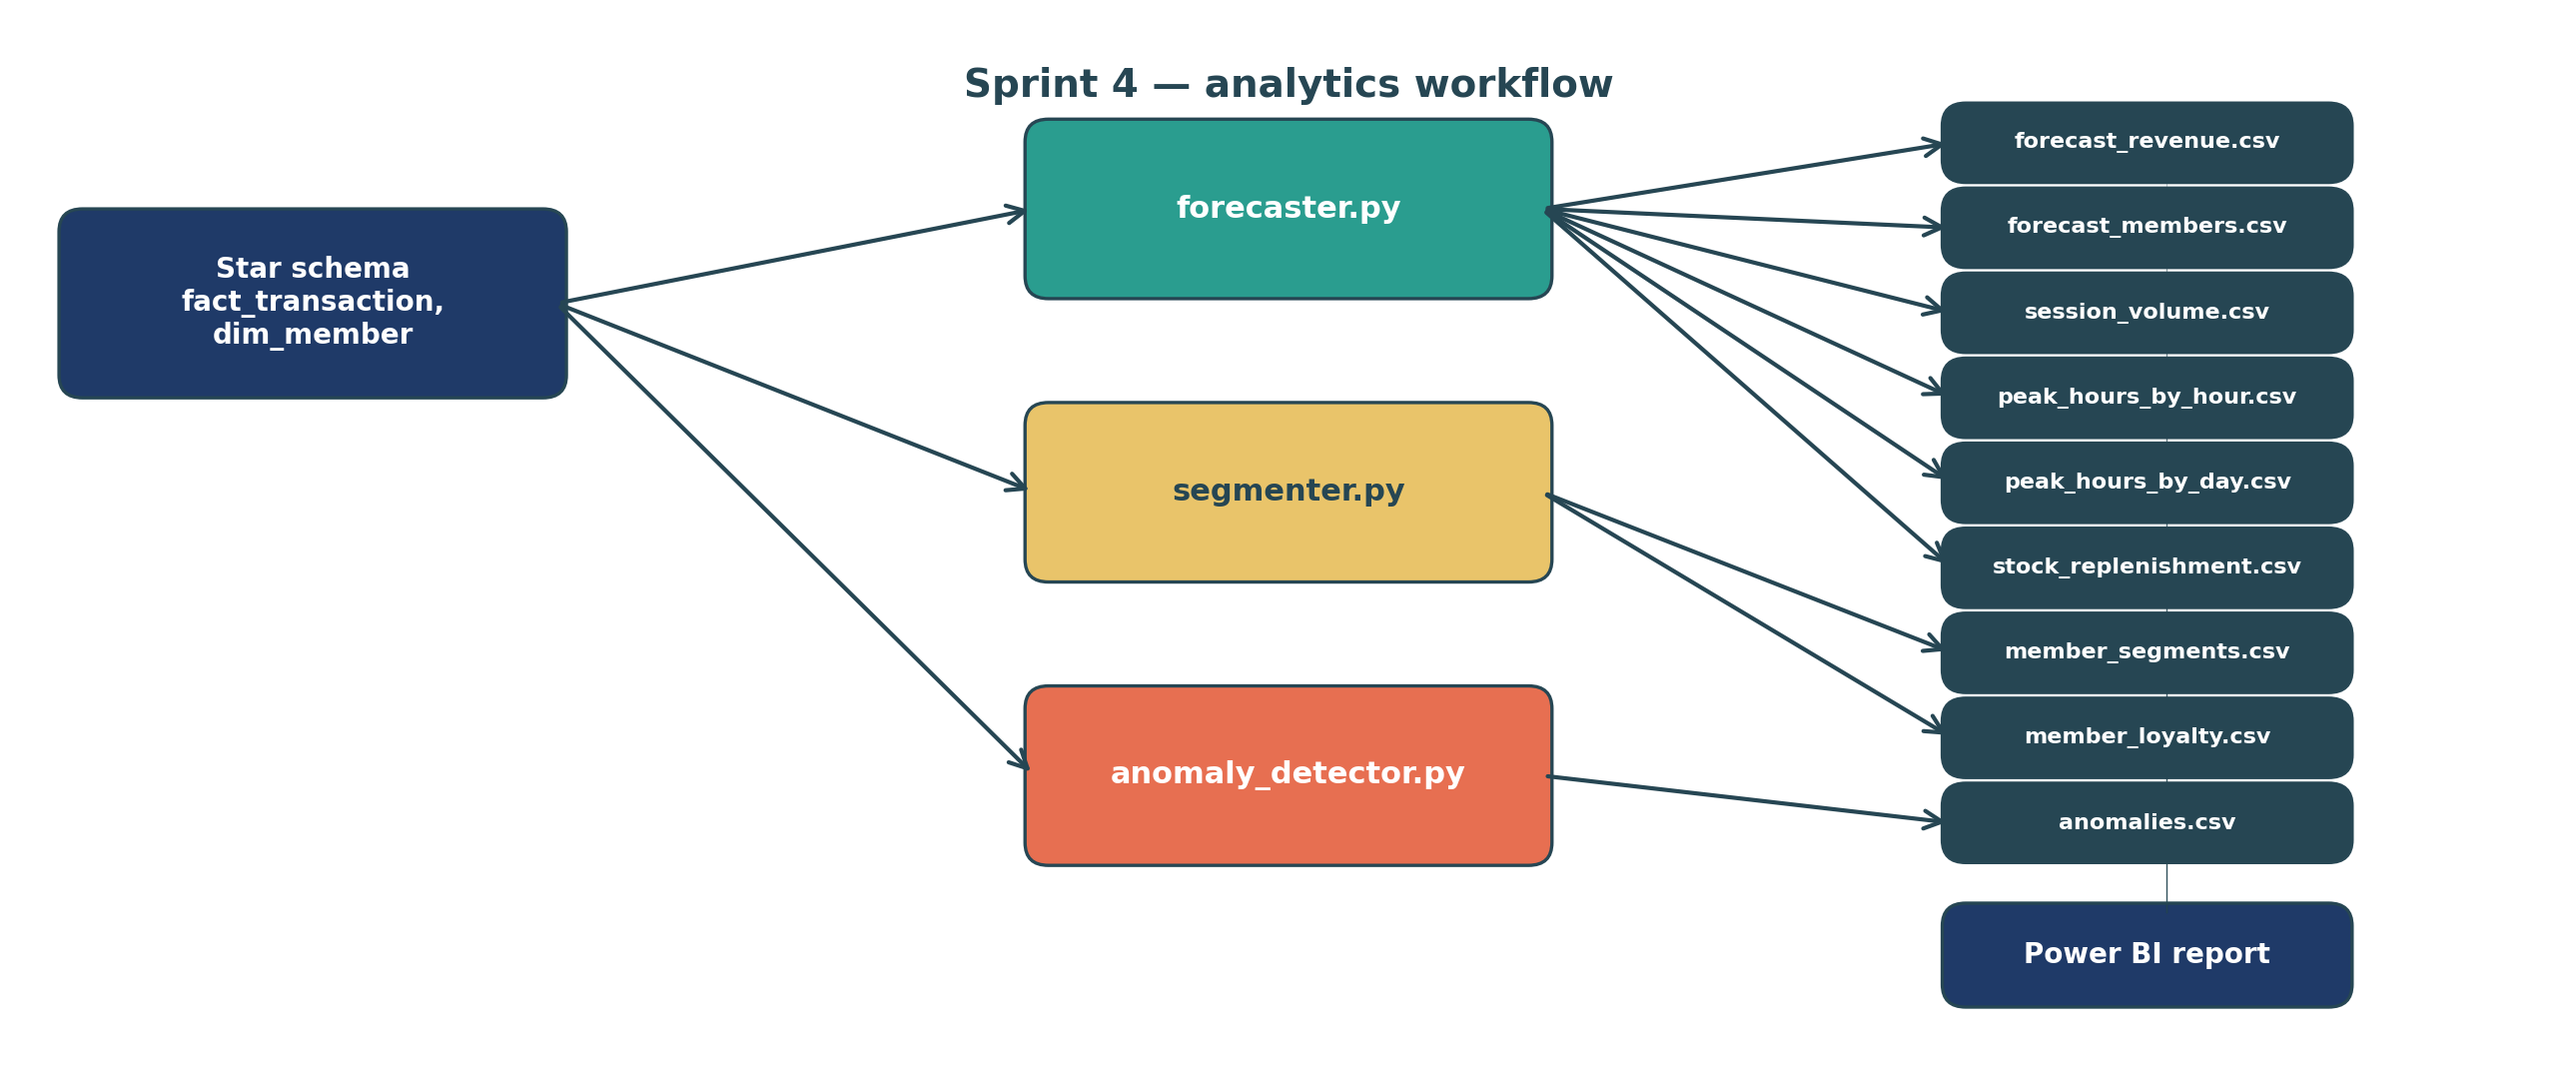
\includegraphics[width=0.90\textwidth]{images/ml_workflow.png}
  \caption{Overview of the Sprint~4 analytics pipeline.\label{fig:ml_workflow}}
\end{figure}

\section{Sprint 4 Backlog}

Table~\ref{tab:sprint4_backlog} lists the tasks committed to this sprint.

\begin{longtable}{>{\bfseries}p{1.3cm} p{4.0cm} p{7.2cm}}
  \caption{Sprint 4 Backlog.\label{tab:sprint4_backlog}} \\
  \toprule
  \textbf{ID} & \textbf{User Story} & \textbf{Tasks} \\
  \midrule
  \endfirsthead
  \toprule
  \textbf{ID} & \textbf{User Story} & \textbf{Tasks} \\
  \midrule
  \endhead
  \bottomrule
  \endfoot

  US-09 & As an owner, I want to see expected revenue for the next 4 weeks and
          3 months so I can plan ahead.
        & Implement \texttt{forecast\_revenue()} using Prophet on daily income
          aggregates; output weekly and monthly projections with confidence
          intervals. \\[4pt]

  US-10 & As an owner, I want to forecast member activity so I know whether
          the loyalty base is growing.
        & Implement \texttt{forecast\_members()} using Prophet on weekly member
          transaction counts; ensure output is a non-negative integer. \\[4pt]

  US-11 & As an owner, I want to know the busiest hours and days so I can
          staff appropriately.
        & Implement \texttt{forecast\_peak\_hours()} computing average transaction
          counts by hour of day and by day of week; export as two separate CSV
          files. \\[4pt]

  US-12 & As an owner, I want to forecast total daily activity volume for the
          next 4 weeks and 3 months.
        & Implement \texttt{forecast\_session\_volume()} using Prophet on the
          daily transaction count as an activity proxy. \\[4pt]

  US-13 & As an owner, I want a restocking recommendation per item so I never
          run out of fast-moving stock.
        & Implement \texttt{forecast\_stock\_replenishment()} computing average
          weekly consumption and suggested order quantities per item. \\[4pt]

  US-14 & As a data analyst, I want to compare two forecasting algorithms so
          the choice of model is objectively justified.
        & Implement SARIMA via \texttt{pmdarima}'s \texttt{auto\_arima} and evaluate
          both Prophet and SARIMA on an 80/20 chronological train/test split;
          report MAE, MAPE, and RMSE for each series. \\[4pt]

  US-15 & As an owner, I want to know which members are my most valuable customers
          so I can target them for promotions.
        & Implement \texttt{segment\_members()} in \texttt{gamefydb/segmenter.py}
          using K-means clustering ($k=4$) on member spend, time, and order features;
          assign human-readable segment labels; export to CSV. \\[4pt]

  US-16 & As an owner, I want to be alerted when a day's revenue or activity was
          abnormally high or low, so I can investigate what happened.
        & Implement \texttt{detect\_anomalies()} in \texttt{gamefydb/anomaly\_detector.py}
          using day-of-week Z-score on three series; classify anomalies by severity;
          export flagged dates to CSV. \\
\end{longtable}

\section{Data Preparation for Machine Learning}

Before any algorithm runs, the cleaned star-schema data needs to be reshaped into
the formats each model expects. This step bridges the relational world of fact tables
and dimension tables and the time-indexed arrays that machine-learning libraries work
with.

\subsection{From Transactions to Daily Series}

The \textit{fact\_transaction} table has one row per individual transaction event.
For time-series forecasting and anomaly detection, what matters is the total for each
calendar day, not the individual events. The pipeline aggregates to daily resolution
using a shared helper function:

\begin{itemize}
  \item \textbf{Revenue series}: filter to income transactions, group by date, sum the
        TND amounts. The result is one row per active day with the total revenue
        earned that day.
  \item \textbf{Session volume series}: count all transactions per date. Because the
        sessions table has no usable timestamps, the daily transaction count is the
        best available proxy for how busy the center was.
  \item \textbf{Member activity series}: count only member-type transactions per date.
        This tracks loyalty card activity separately from walk-in cash customers.
\end{itemize}

In all three cases the result is a two-column DataFrame with a date column
(\texttt{ds}) and a value column (\texttt{y}) --- the exact format Prophet expects.

\subsection{Weekly Aggregation for Member Activity}

Member transactions are sparse at the daily level: on a typical day, only two to five
are recorded. When Prophet models numbers this small, the lower bound of its confidence
interval goes negative --- which is meaningless for a transaction count.

The fix is to aggregate to weekly totals before fitting. Each week's count is large
enough for Prophet to estimate uncertainty reliably, and the lower bound stays
non-negative. All member forecast values are clipped at zero and rounded to the
nearest integer before export.

\subsection{Feature Normalisation for K-Means}

K-means measures the Euclidean distance between data points to assign clusters. This
creates a scale problem: if total spend ranges from 0 to 2000~TND and session duration
from 0 to 3000~minutes, the algorithm weights spend more heavily --- not because it
is more important, but because the numbers are larger.

StandardScaler solves this by shifting each feature to zero mean and scaling it to
unit standard deviation. After normalisation, a 200~TND difference in spending and a
30-minute difference in session time represent the same magnitude of deviation. Both
features contribute equally to the distance calculation.

\subsection{Weekday Grouping for Anomaly Detection}

Anomaly detection groups the existing daily values by day of the week before comparing
them. All Mondays are compared together, all Saturdays together, and so on.

This matters because a gaming center has a strong weekly rhythm: Saturdays are
consistently busier than Tuesdays. Comparing a Saturday against the average of all
days would flag almost every Saturday as anomalous --- which tells the owner nothing
useful. Grouping within weekdays means the baseline reflects what is normal for that
specific day, not the overall daily average.

\begin{figure}[H]
  \centering
  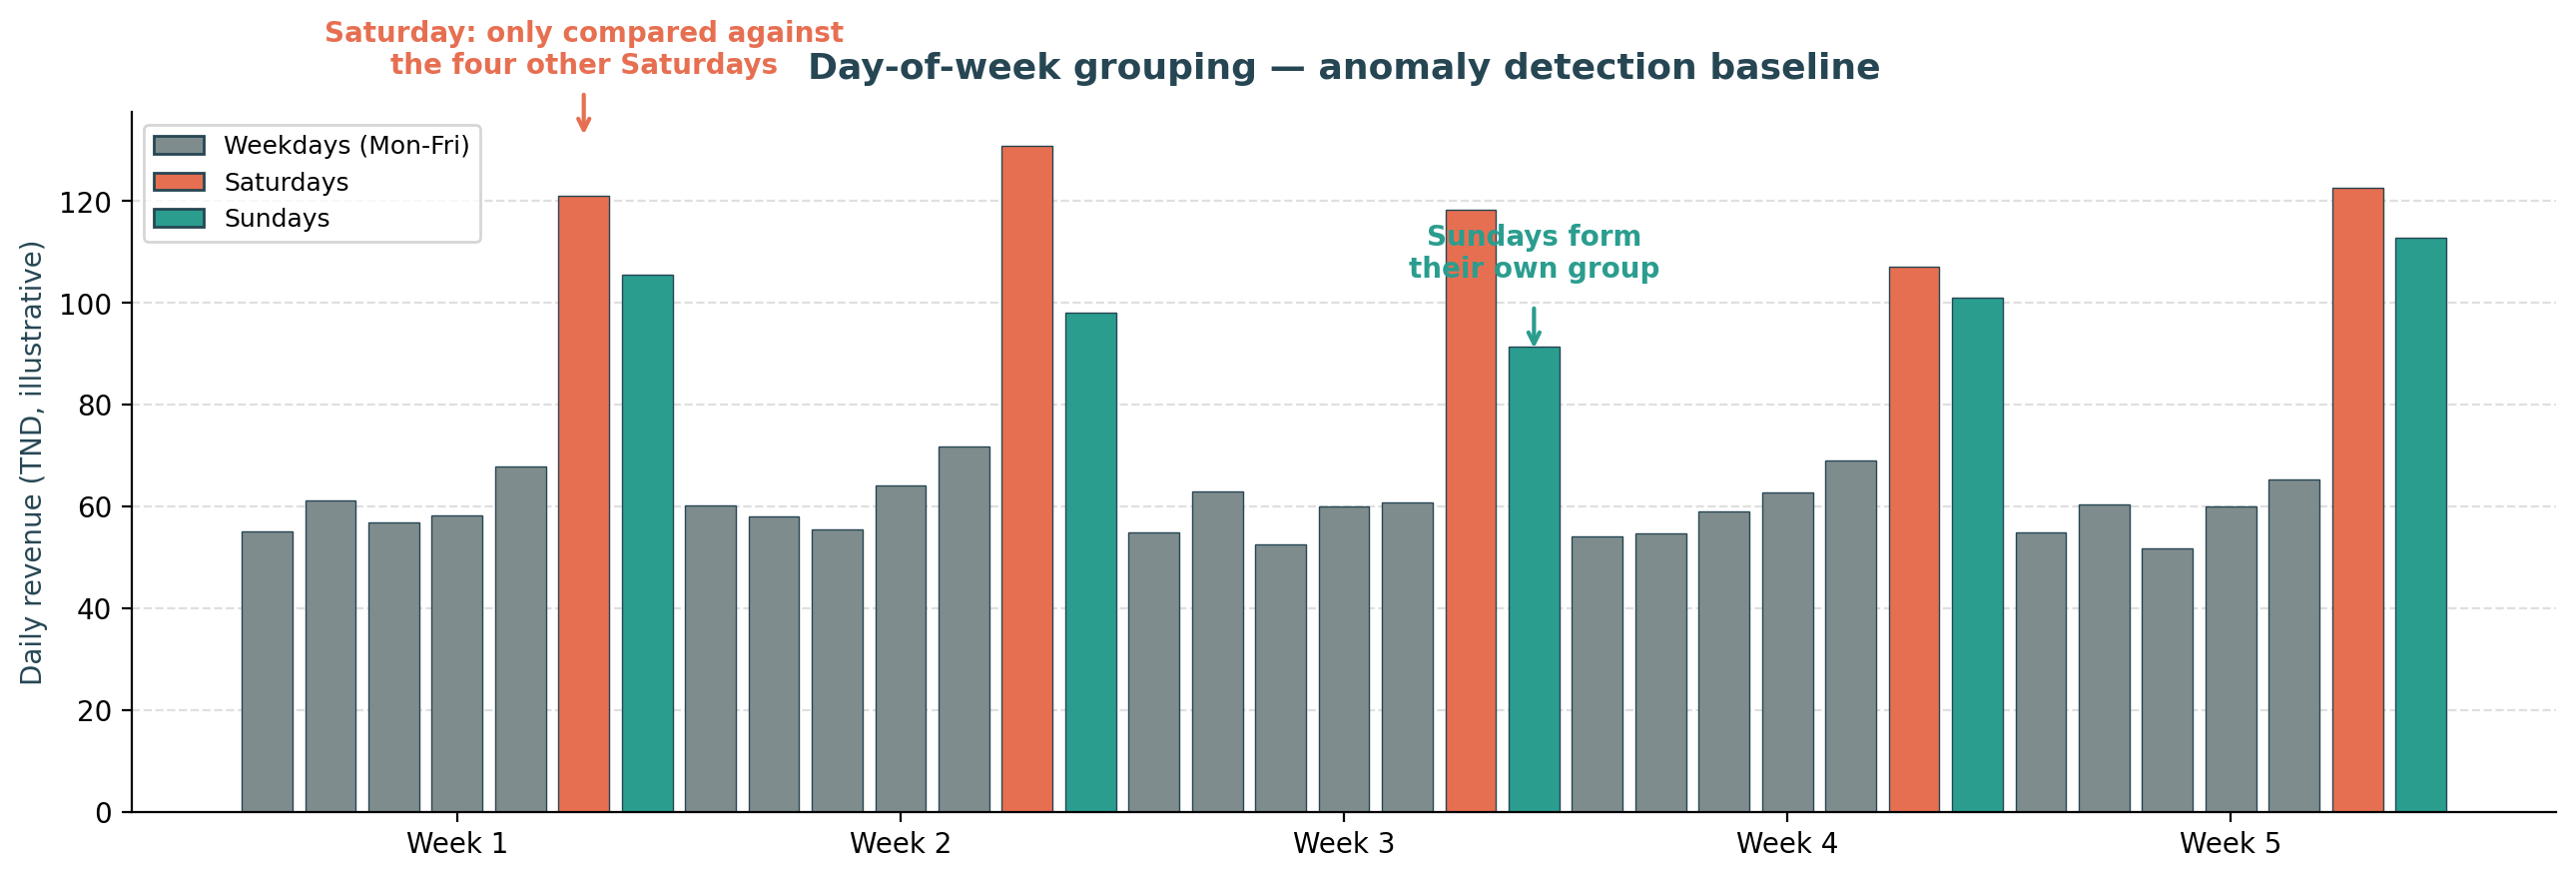
\includegraphics[width=0.85\textwidth]{images/weekday_grouping.png}
  \caption{Day-of-week grouping: each day is compared only against historical values
           from the same weekday.\label{fig:weekday_grouping}}
\end{figure}

\subsection{Stationarity Analysis}

Before fitting any forecasting model, it is essential to verify whether the time series
are \textbf{stationary} --- that is, whether their statistical properties (mean, variance)
remain constant over time. Non-stationarity, caused by trends or varying variance, can
lead to unreliable model estimates if left unaddressed.

Two complementary approaches were used to study stationarity, following standard practice
in time-series analysis:

\begin{itemize}
  \item \textbf{Graphical method}: visual inspection of the raw series together with a
        centered rolling mean to detect any visible trend or changing variance.
  \item \textbf{Statistical test}: the Augmented Dickey-Fuller (ADF) test provides
        a formal hypothesis test for the presence of a unit root.
\end{itemize}

Figure~\ref{fig:stationarity_rolling} presents the graphical analysis. The left
column shows each raw series with a centered rolling mean: the mean clearly
drifts upward for member activity, the revenue series shows long bursts of
variance around the Eid and back-to-school weeks, and the session-volume
rolling mean climbs through 2025. To produce a visually stable counterpart, a
two-step stabilization is applied: $\log(1+y_t)$ to compress the bursts in
variance, followed by a first-difference $\Delta y_t = y_t - y_{t-1}$ to
remove the trend. The right column shows the result --- a series hovering
tightly around zero with a roughly constant band, the visual hallmark of a
stationary series.

\begin{figure}[H]
  \centering
  
\includegraphics[width=0.95\textwidth]{stationarity_rolling.png}
  \caption{Graphical stationarity check, before (left) and after (right) the
           $\log(1+y)$+first-difference stabilization. The right column hovers
           around zero with a constant band, confirming that the trend and
           variance bursts visible in the raw series have been
           removed.\label{fig:stationarity_rolling}}
\end{figure}

\subsubsection*{The ADF Test}

The ADF test evaluates two hypotheses:
\begin{itemize}
  \item $H_0$: the series contains a unit root and is therefore non-stationary.
  \item $H_1$: the series has no unit root and is stationary.
\end{itemize}
The decision rule uses a significance level of $\alpha = 0.05$: if the p-value is below
$0.05$, $H_0$ is rejected and the series is considered stationary.

The test was applied to all three series used in the forecasting step --- daily
revenue (TND), daily session volume, and weekly member activity --- both before
and after the stabilization step. The results are shown in
Table~\ref{tab:adf_results}.

\begin{table}[H]
  \centering
  \begin{tabular}{lrrcrr}
    \hline
                                & \multicolumn{2}{c}{\textbf{Raw series}} & &
                                  \multicolumn{2}{c}{\textbf{After log + diff}} \\
    \cline{2-3} \cline{5-6}
    \textbf{Series}             & \textbf{ADF statistic} & \textbf{p-value} & &
                                  \textbf{ADF statistic} & \textbf{p-value} \\
    \hline
    Revenue (TND, daily)        & $-5.213$ & $<0.001$ & & $-13.530$ & $<0.001$ \\
    Session volume (daily)      & $-4.973$ & $<0.001$ & & $-12.146$ & $<0.001$ \\
    Member activity (weekly)    & $-5.957$ & $<0.001$ & &  $-6.430$ & $<0.001$ \\
    \hline
  \end{tabular}
  \caption{ADF stationarity test results before and after
           $\log(1+y)$+first-difference stabilization. All six tests reject
           $H_0$; the stabilized statistics are roughly twice as decisive for
           the daily series. Source:
           \texttt{output/forecasts/stationarity\_tests.csv}.%
           \label{tab:adf_results}}
\end{table}

\subsubsection*{Handling Non-Stationarity}

The stabilization step is used as a diagnostic only; the forecasting models
themselves are fitted on the raw series. Both Prophet and SARIMA are designed
to work directly with non-stationary real-world data:

\begin{itemize}
  \item \textbf{Prophet} fits a piecewise linear trend component that explicitly models
        long-run growth or decline. The series does not need to be pre-differenced or
        log-transformed --- the model absorbs the non-stationarity through its
        trend term.
  \item \textbf{SARIMA} (via \texttt{pmdarima}'s \texttt{auto\_arima}) automatically
        selects the integration order~$d$ (and $D$ for seasonal integration) by testing
        several candidates and picking the one that minimises AIC. The differencing is
        applied internally before parameter estimation, so the raw series can be fed
        directly without manual pre-processing.
\end{itemize}

This separation --- stabilization for analysis, raw input for the models ---
matches the standard practice in applied time-series work: the ADF and rolling
plots document the statistical properties of the data, while Prophet and
auto\_arima handle whatever trend or unit-root behaviour is present in the raw
series at fit time.

\section{Forecasting Technology}

\subsection{Why Prophet}

Three of the five forecast outputs use \textbf{Prophet}, an open-source time-series
library developed by Meta. It was chosen for practical reasons: it handles the kind of
data a small business produces without requiring manual calibration.

\begin{itemize}
  \item \textbf{Missing dates}: the center has no transactions on some days. Prophet
        treats those as gaps, not as zeros.
  \item \textbf{Weekly seasonality}: Prophet detects the weekend peak automatically,
        without being told which days are weekends.
  \item \textbf{Confidence intervals}: alongside the point forecast (\texttt{yhat}),
        Prophet produces an 80\% confidence band (\texttt{yhat\_lower} and
        \texttt{yhat\_upper}). This gives the owner a range to plan around rather than
        a single number.
  \item \textbf{No manual tuning}: the model works out of the box for a
        single-location business time series.
\end{itemize}

Under the hood, Prophet fits an additive decomposition:
\[
  y(t) = \text{trend}(t) + \text{seasonality}(t) + \epsilon_t
\]
The trend is a piecewise linear function that adapts to growth or decline over time.
The seasonality is a Fourier-series approximation of weekly and yearly cycles.
The residual $\epsilon_t$ captures everything else.

\begin{figure}[H]
  \centering
  
\includegraphics[width=0.88\textwidth]{prophet_revenue_forecast.png}
  \caption{Prophet revenue forecast: historical data, 4-week and 3-month projections,
           and 80\% confidence band.\label{fig:prophet_forecast}}
\end{figure}

\subsection{SARIMA as a Comparison Algorithm}

To validate the choice of Prophet objectively, \textbf{SARIMA} (Seasonal AutoRegressive
Integrated Moving Average) was implemented as a comparison. SARIMA is the classical
standard for seasonal time-series forecasting, and it was deliberately chosen because
it also handles seasonality --- comparing Prophet against a model that ignores
seasonality would make the result unfair and academically weak.

SARIMA has six parameters: $p$, $d$, $q$ (non-seasonal) and $P$, $D$, $Q$ (seasonal),
plus a seasonal period~$m$. Selecting these manually is time-consuming and introduces
bias. The implementation uses \texttt{pmdarima}'s \texttt{auto\_arima}, which tests
combinations automatically and selects the best by AIC (Akaike Information Criterion).
The seasonal period is $m=7$ for daily series (one week) and $m=4$ for weekly series
(one month).

\subsection{Evaluation Methodology --- 80/20 Chronological Split}

Both algorithms are evaluated on the same data using a \textbf{chronological 80/20
split}: the first 80\% of the historical series trains the model and the final 20\% is
held out as the test set. The model then predicts the test period, and those predictions
are compared against the real values from the source files.

The split must be chronological. A random split would allow the model to train on
data from March to predict February, which is not how forecasting works in practice.
The test set must always come after the training set in time.

\begin{figure}[H]
  \centering
  
\includegraphics[width=0.80\textwidth]{train_test_split.png}
  \caption{Chronological 80/20 train/test split used for model
           evaluation.\label{fig:split}}
\end{figure}

Three metrics are computed for each algorithm and each series:

\begin{itemize}
  \item \textbf{MAE} (Mean Absolute Error) --- the average absolute gap between
        predicted and actual values, in the same unit as the data (TND for revenue,
        integer count for activity). Straightforward to interpret: on average, the
        model was off by this amount.
  \item \textbf{MAPE} (Mean Absolute Percentage Error) --- the average percentage gap.
        This is the primary decision metric because it is scale-independent: a 12\%
        error on revenue and a 12\% error on session count represent the same quality,
        even though the raw numbers are very different. A MAPE below 10\% is good,
        below 20\% is acceptable, and above 20\% is poor.
  \item \textbf{RMSE} (Root Mean Squared Error) --- similar to MAE but squaring errors
        before averaging gives heavier weight to large individual mistakes. A large gap
        between RMSE and MAE means a few predictions were very far off; a small gap
        means errors are consistent.
\end{itemize}

The algorithm with the lower wMAPE is declared the winner for each series. A third
comparator, \textbf{XGBoost} with lagged features (lag 1, lag 7, lag 14, rolling
7- and 14-day means, plus calendar and holiday-proximity features), was also added
to the evaluation harness. The full comparison across the three algorithms is
reported in Section~\ref{sec:data_journey}, after the data-engineering work that
made the comparison meaningful in the first place.

\medskip
\noindent\textbf{A note on wMAPE versus arithmetic MAPE.}
The standard MAPE definition --- the mean of $|y_i - \hat{y}_i| / y_i$ --- breaks down
when individual $y_i$ values approach zero, because one near-zero day can produce a
percentage error of several thousand percent and dominate the average. Gaming-center
data has many quiet days, and the early evaluation runs were dominated by these
spurious extremes rather than by the model's real behaviour. The pipeline therefore
reports \textbf{weighted MAPE} (wMAPE), defined as $\text{MAE} / \overline{y} \times 100$,
where $\overline{y}$ is the mean of the actual values across the test set. This is
the same total-error / total-actual ratio used by Kaggle and Meta's own Prophet
publications, and it is stable for series with low-volume days.

\section{From Limited Real Data to a Trainable Forecast}\label{sec:data_journey}

When the forecasting work began, the dataset covered roughly seven months ---
from the start of operations in September~2025 through the end of March~2026.
For a model whose main strength is detecting yearly cycles, this is short.
Prophet can technically fit on any range, but with no Christmas, no Eid al-Fitr,
and no summer captured twice, the yearly seasonality component is little more
than an extrapolation of seven months of weekly variation. The first evaluation
runs reflected this: weighted MAPE values above 65\,\% on every series, with
Prophet barely beating a naive day-of-week baseline.

This section documents the work done to bring those numbers into a usable
range. None of it was planned at the start of the sprint --- each step
followed from looking at where the model was wrong and asking why.

\subsection{First Attempt: Synthetic History Extension}

The most direct fix was to lengthen the training history. A synthetic data
generator was written (in \texttt{gamefydb/data\_generator.py}) to produce
realistic transaction-level records for the periods before September~2025.
It was deliberately not a naive repeat of historical averages. The generator
samples per-month revenue distributions from the real data using a bootstrap
with day-of-week adjustment; it applies an autoregressive weekly state with
$\alpha=0.45$ so weeks correlate with their predecessors instead of being
independent draws; and it draws transaction times from the empirically observed
hourly profile.

A first version generated twelve months going back from September~2024,
combined with the real data to produce roughly eighteen months of training
material. Inspecting the output side by side with the real files showed that
transaction counts, revenue distributions, and weekly rhythms matched well.

The forecast accuracy improved, but only modestly. Prophet was now seeing one
full annual cycle, yet its predictions for the March~2026 test window were
systematically too low. The worst-predicted day of the entire test set was
March~31, 2026 --- where the actual revenue was nearly four times the predicted
value. That date is Eid al-Fitr.

\subsection{The Ramadan and Eid Discovery}

Two problems were happening at once. The first was in the holiday-boost
dictionary. Its keys were two-tuples of \texttt{(month, day)}, which meant
the same boost was applied to the same calendar date every year. But Eid al-Fitr
2025 fell on March~31, while Eid al-Fitr 2026 fell on March~21. Half the time
the boost was applied on the wrong day; the other half it was applied to a
date that had no holiday at all. Prophet was learning, in effect, that
"March~31 is busy" --- which was true for one year and meaningless for the
next.

The second problem was the shape of Ramadan itself. The generator had a
Boolean \texttt{\_in\_ramadan} helper that shifted the hourly transaction
distribution toward the post-iftar evening hours, but it did not change the
daily revenue volume at all. Real gaming centers in Tunisia do not run flat
through Ramadan: the first week is typically quieter than normal as people
adjust to the new rhythm, and the final week --- particularly the last ten
days, which include Layilatul Qadr --- ramps sharply upward toward Eid. The
model had no way to learn this because the signal was not in the training
data.

\subsection{Engineering the Holiday Signal}

Fixing the data took five focused changes. Each one was written test-first:
a failing unit test specified the expected behaviour before any production
code was touched. The resulting 26-test suite in
\texttt{tests/test\_data\_generator.py} covers the helper functions in
isolation and runs an end-to-end integration check that verifies synthetic
Eid-day revenue is materially higher than surrounding baseline.

\paragraph{Year-keyed holiday boost.} The dictionary keys became three-tuples
of \texttt{(year, month, day)}, populated by a helper that loops over the years
2022--2026 and stamps each year's specific Islamic dates exactly once. The dates
were synced with the same calendar Prophet receives as its \texttt{holidays}
argument, eliminating the cross-year leak permanently.

\paragraph{Extended Ramadan periods.} The \texttt{\_RAMADAN\_PERIODS} list was
extended to cover 2022 through 2026 (one window per year). The 2026 end-date
was nudged from March~17 to March~19 so the window actually reaches Eid
al-Fitr on March~21 --- the prior end-date left a two-day gap between the end
of Ramadan and Eid where the model saw a sudden drop followed by an unexplained
spike.

\paragraph{Daily ramp inside Ramadan.} A new \texttt{\_ramadan\_daily\_mul}
helper computes a daily multiplier that increases monotonically through the
month: starting near 0.85 for the first 40\,\% of days, holding around 1.0
across the middle, and ramping to 1.5 by the final day. This captures the
"quiet start, busy finish" pattern observed in real Ramadan data.

\paragraph{Eid-week cluster pattern.} A second helper,
\texttt{\_eid\_week\_pattern}, applies a decaying spike on Eid+1, Eid+2, and
Eid+3 at 80\,\%, 60\,\%, and 40\,\% of the Eid-day boost respectively. This
reflects the observation that gaming centers remain unusually full for several
days after Eid, not just on the day itself.

\paragraph{Wider augment window.} With the holiday machinery now working
correctly, the synthetic-history range was extended from twelve months to
twenty-four months, producing data going back to September~2022. Combined
with the existing extended window and the real data, the training set grew
to 44~months --- long enough for Prophet to see three complete Ramadan cycles
(2023, 2024, 2025) before the test set begins.

\subsection{Verification}

After regenerating the data, the Eid al-Fitr 2025 daily revenue in the
synthetic series jumped from a baseline of roughly 150~TND to 956~TND on
March~31, with Eid+1, Eid+2, and Eid+3 at 946, 720, and 597~TND --- exactly
the decay shape the helper was designed to produce. The anomaly detector
confirmed this independently: when run on the regenerated data, it flagged
March~31, 2025 with a Z-score of $+5.74$, classifying it as a severe high
outlier. The signal was now unambiguously present in the training data.

A constant invariant throughout this work was that the real \texttt{.xls}
source files in \texttt{excel/} were never modified. All synthetic content
was written to \texttt{excel/extended\_*.xlsx} and \texttt{excel/augment/}
alongside the originals. The git status on \texttt{excel/} was checked after
each regeneration to confirm no real-data files had been touched.

\subsection{Prophet Hyperparameter Tuning}

With the data signal corrected, attention turned to Prophet itself. Three
changes were applied:

\begin{itemize}
  \item Islamic-holiday entries for 2022 and 2023 were added to the
        forecaster's holiday calendar so that the new augment years were
        no longer "blind" to the spikes embedded in their synthetic data.
  \item The upper window on every Eid was extended from two to three days
        to match the Eid+1..Eid+3 cluster shape now present in the data.
  \item \texttt{holidays\_prior\_scale} was increased from the default value
        of~10 to~20, giving Prophet stronger evidence to weight holiday
        effects against the underlying trend.
\end{itemize}

A fourth experiment --- raising \texttt{changepoint\_prior\_scale} from~0.05
to~0.1 --- was reverted after testing. It improved the daily revenue series
by a small margin but regressed the weekly member-activity series, which only
has 153~training points and overfits under the more flexible setting.

These changes together brought the daily-resolution wMAPE values from roughly
56\,\% down to around 52\,\% on revenue and session volume. Acceptable as a
relative improvement, but still well above the 25--30\,\% range that would
make the forecast useful for actual planning decisions.

\subsection{Choosing the Right Resolution}

Looking at the residual distributions explained where the remaining error was
coming from. Daily revenue had a coefficient of variation of roughly~0.6 ---
the standard deviation was nearly two-thirds of the mean. Part of that
variation was holiday and weekend structure that Prophet could in principle
learn. The other part was true day-to-day noise: cashier shift differences,
weather, a viral content creator stream, a local football match. No model
trained only on the calendar can predict those.

A key observation followed from this: the deliverable from the forecasting
module was already weekly and monthly aggregates --- the daily numbers were
an internal step, never exposed to the dashboard. The natural fix was to
evaluate on the same resolution the business actually consumes. The
\texttt{\_evaluate\_prophet}, \texttt{\_evaluate\_sarima}, and
\texttt{\_evaluate\_xgboost} helpers were extended to accept a weekly-aggregated
series, and the evaluation pipeline was switched accordingly.

The improvement was substantial. Revenue Prophet dropped from 52.6\,\% to
38.9\,\% wMAPE in a single change. Session volume Prophet dropped from
52.5\,\% to 44.0\,\%. The natural averaging at weekly resolution had absorbed
most of the irreducible daily noise.

\subsection{Log Transformation for Multiplicative Variance}

Even at weekly resolution, the residuals had a recognisable shape: small
absolute errors on quiet weeks, very large errors on Eid weeks. The weekly
revenue series ranged from 224~TND to 4{,}642~TND --- a 20-fold spread.
Prophet's additive decomposition struggles with this because the same
percentage error produces a much larger absolute error on big weeks than
on small ones. Fitting on $\log(1+y)$ converts the multiplicative variance
into additive form; the predictions are transformed back with $\exp(\hat{y})-1$
before the metrics are computed.

Adding the log transformation to the weekly Prophet evaluation produced a
further drop. Revenue moved from 38.9\,\% to 29.7\,\% wMAPE. Session volume
moved from 44.0\,\% to 36.8\,\%. The member-activity series did not benefit
from the transformation and was left in raw scale --- its weekly mean is
around ten transactions, below the regime where log compression helps.

\subsection{Final Evaluation Results}

Table~\ref{tab:forecast_comparison_final} shows the final weighted-MAPE
figures, computed on an 80/20 chronological train/test split at weekly
resolution, with log transformation applied to revenue and session volume.
All three algorithms --- Prophet, SARIMA, and XGBoost --- are evaluated on
the same train/test sets.

\begin{table}[H]
  \centering
  \caption{Final evaluation results. Weekly resolution, 80/20 chronological
           split, 154 train weeks / 39 test weeks. Best per series in
           \textbf{bold}.\label{tab:forecast_comparison_final}}
  \begin{tabular}{llrrrl}
    \toprule
    \textbf{Series} & \textbf{Algorithm} & \textbf{MAE} & \textbf{wMAPE} &
    \textbf{RMSE} & \textbf{Verdict} \\
    \midrule
    \multirow{3}{*}{Revenue (TND, weekly)}
      & \textbf{Prophet} & \textbf{470.1} & \textbf{29.7\,\%} & \textbf{644.8} & Acceptable \\
      & SARIMA  & 585.1 & 37.0\,\% & 706.7 & Acceptable \\
      & XGBoost & 732.6 & 46.4\,\% & 886.2 & Acceptable \\
    \midrule
    \multirow{3}{*}{Session volume (weekly)}
      & Prophet & 41.2 & 36.8\,\% & 52.4 & Acceptable \\
      & \textbf{SARIMA}  & \textbf{40.7} & \textbf{36.4\,\%} & \textbf{50.3} & Acceptable \\
      & XGBoost & 50.8 & 45.4\,\% & 64.8 & Acceptable \\
    \midrule
    \multirow{3}{*}{Member activity (weekly)}
      & \textbf{Prophet} & \textbf{5.3} & \textbf{52.5\,\%} & \textbf{9.2} & Poor \\
      & SARIMA  & 5.9 & 59.2\,\% & 9.0 & Poor \\
      & XGBoost & 5.5 & 55.9\,\% & 9.4 & Poor \\
    \bottomrule
  \end{tabular}
\end{table}

Prophet wins on revenue and on member activity; SARIMA wins on session
volume by the smallest possible margin (0.4~percentage points). On the two
daily-derived weekly series, both Prophet and SARIMA land in the acceptable
30--40\,\% range. The member-activity series remains poor: with a weekly
mean of around ten transactions and only 39~test weeks available, the
wMAPE denominator is small enough that even reasonable absolute errors
translate to high percentage figures. Improving this further would require
either monthly aggregation (fewer points but more stable means) or several
more months of operational history --- neither of which fit in the sprint
scope.

For context: the journey from the very first evaluation run to this table
moved revenue Prophet wMAPE from roughly 67\,\% on the original seven-month
dataset to 29.7\,\% on the final 44-month dataset --- a more than two-fold
improvement. Most of that gain came from honest data engineering (fixing the
holiday signal, extending the training window) and from a deliberate choice
of evaluation resolution, rather than from aggressive hyperparameter search.

\subsection{Error Decomposition: Where Does the Residual Error Live?}

A natural follow-up question, given how much of the work focused on Ramadan
and Eid, is whether the residual headline wMAPE is concentrated in those
weeks. To answer it, the test set was tagged with a binary
\textit{holiday-cluster} label: any week containing a Ramadan day, an Eid day,
or one of Eid+1, Eid+2, or Eid+3 was marked as holiday; all others as
ordinary. The error was then recomputed on each subset separately while
keeping the same trained model and the same predictions --- nothing was
re-fit. The output is written to
\texttt{output/forecasts/error\_decomposition.csv}.

\begin{table}[H]
  \centering
  \caption{Error decomposition on the test set: ordinary weeks vs.\ holiday-cluster
           weeks (Ramadan + Eid+0..+3). \emph{Share of total error} is the
           share of absolute test-set error contributed by each
           subset.\label{tab:error_decomposition}}
  \begin{tabular}{llrrrrr}
    \toprule
    \textbf{Series} & \textbf{Model} &
    \textbf{wMAPE} & \textbf{Ordinary} & \textbf{Holiday} &
    \multicolumn{2}{c}{\textbf{Share of total error}} \\
    \cmidrule(lr){6-7}
    & & \textbf{(full)} & \textbf{(33 w.)} & \textbf{(6 w.)} &
    \textbf{Ord.} & \textbf{Hol.} \\
    \midrule
    \multirow{3}{*}{Revenue}
      & \textbf{Prophet} & 29.8\,\% & 34.4\,\% & \textbf{9.2\,\%}  & 94.2\,\% & 5.8\,\% \\
      & SARIMA           & 37.0\,\% & 39.5\,\% & 26.1\,\% & 86.9\,\% & 13.1\,\% \\
      & XGBoost          & 46.4\,\% & 52.4\,\% & 20.1\,\% & 92.0\,\% & 8.0\,\% \\
    \midrule
    \multirow{3}{*}{Session volume}
      & \textbf{Prophet} & 36.8\,\% & 42.1\,\% & \textbf{11.1\,\%} & 94.9\,\% & 5.1\,\% \\
      & SARIMA           & 36.4\,\% & 37.4\,\% & 31.4\,\% & 85.3\,\% & 14.7\,\% \\
      & XGBoost          & 45.4\,\% & 52.7\,\% &  9.9\,\% & 96.3\,\% & 3.7\,\% \\
    \midrule
    \multirow{3}{*}{Member activity}
      & Prophet & 52.5\,\% & 53.2\,\% & 50.2\,\% & 78.5\,\% & 21.5\,\% \\
      & SARIMA  & 59.2\,\% & 63.3\,\% & 44.8\,\% & 83.1\,\% & 16.9\,\% \\
      & XGBoost & 55.9\,\% & 59.0\,\% & 45.3\,\% & 82.0\,\% & 18.0\,\% \\
    \bottomrule
  \end{tabular}
\end{table}

The result was the opposite of what was initially expected. The hypothesis
going in was that holiday weeks would still dominate the residual error ---
those are the spikes the model has to predict, and a small miss there
translates to a large absolute number. In practice, after the data
engineering and the calendar synchronisation, Prophet now fits holiday weeks
\emph{better} than ordinary weeks: wMAPE on the six holiday-cluster weeks is
9.2\,\% for revenue and 11.1\,\% for session volume, while ordinary weeks
sit at 34.4\,\% and 42.1\,\% respectively. Across the full test set, only
roughly 5--6\,\% of the absolute error on revenue and sessions comes from
the holiday subset.

This carries a useful diagnostic implication. The remaining headline
wMAPE is no longer about holidays --- it is week-to-week base-rate noise.
The kind of variation that drives an ordinary Saturday from 250\,TND to
400\,TND for reasons the calendar cannot capture: a viral live stream, a
local football match, a power outage, a popular tournament announced two
days earlier. None of these are predictable from \texttt{ds} alone. Closing
that gap further would require non-calendar regressors (external event
flags, weather data, exogenous demand signals) rather than more
holiday-engineering work, which has effectively reached diminishing returns.

The member-activity decomposition tells a different story: ordinary and
holiday-cluster wMAPE are both around 50\,\%, with no meaningful gap.
This series is small-sample-limited, not signal-limited. A 39-week test
horizon with a weekly mean of about ten transactions does not have enough
data for any of the three algorithms to outperform a roughly trend-only
fit. Adding a year or two of operational history would help more than any
model change.

A caveat on the holiday subset: with only six weeks in it, the wMAPE on
that subset is statistically noisy --- one bad week swings the percentage
visibly. The figures should be read as an order-of-magnitude diagnostic,
not as precision measurements.

\begin{figure}[H]
  \centering
  
\includegraphics[width=0.95\textwidth]{accuracy_revenue_prophet.png}
  \caption{Final Prophet revenue forecast on weekly resolution with log
           transformation. Light-blue: historical training data; black:
           actual test-period values; green: Prophet prediction with 80\,\%
           confidence band.\label{fig:final_revenue_prophet}}
\end{figure}

\begin{figure}[H]
  \centering
  
\includegraphics[width=0.85\textwidth]{model_comparison_bar.png}
  \caption{wMAPE comparison across the three algorithms and three forecast
           series at the final tuned configuration.\label{fig:final_comparison}}
\end{figure}

\subsection{Weather as a Non-Calendar Regressor}

The error decomposition above pointed in a specific direction: the remaining
headline wMAPE on revenue and session volume is no longer explained by
holidays, and closing the gap further would require exogenous signals
that the calendar cannot supply. Weather is the most obvious candidate.
A rainy Saturday in Tunis pulls customers away from outdoor activities and
toward indoor venues; an unusually hot day in July drives the same shift
through a different mechanism (escape from heat into air-conditioned space).
Neither effect is encoded anywhere in \texttt{ds}.

A new module \texttt{gamefydb/weather.py} was added to fetch daily Tunis
weather from the Open-Meteo Archive API (latitude~36.81, longitude~10.18).
Two features are extracted per day: \texttt{temp\_max\_c} (maximum
temperature in Celsius) and \texttt{precip\_mm} (precipitation in
millimetres). Results are cached locally to
\texttt{excel/weather\_tunis.parquet} so repeated pipeline runs hit the
network zero times. For dates beyond the cache, the module falls back to a
climatological average computed over the cached history --- mean
temperature and precipitation grouped by \texttt{(month, day)}.

The two features are wired into Prophet via \texttt{add\_regressor()} and
into XGBoost as additional columns alongside the existing lagged and
calendar features. SARIMA was left unchanged for the same reason it lacks
a holiday calendar in this implementation: the SARIMAX extension that
accepts exogenous variables would close the gap, but adding it here did
not justify the implementation effort for a comparator that is already
outperformed by Prophet. Member activity was likewise left out: at weekly
resolution and a mean of ten transactions, the daily weather signal
disappears in the aggregation.

\paragraph{A methodological pitfall encountered en route.}
The first attempt to validate the regressor used synthetic data in which
weather had \emph{already} been baked into the daily revenue target via a
multiplicative factor (\textit{precip} $> 2$\,mm reduced the day by
10\,\%; \textit{temp\_max} $> 33$\,\degree C raised it by 8\,\%). The
intent was to give the model a coherent weather signal across the full
18-month training window rather than only the real Sep~2025+ tail.
The result was the opposite of what was expected: adding weather as a
regressor on top of weather-injected synthetic data made every metric
slightly worse. The cause turned out to be double-counting --- the same
effect was present both in the target $y$ and in the regressor, so the
regressor was fitting noise around an already-explained component and
adding variance without adding bias reduction. Regenerating the synthetic
data without the weather multiplier and re-evaluating produced the
opposite verdict, which is what is reported below. The lesson is general:
when injecting an artificial signal into synthetic training data,
\emph{do not} simultaneously expose that signal as a regressor.

\begin{table}[H]
  \centering
  \caption{Weather regressor evaluation. Same weekly 80/20 split as
           Table~\ref{tab:forecast_comparison_final}. Negative
           $\Delta$~wMAPE indicates improvement.\label{tab:weather_regressor}}
  \begin{tabular}{llrrr}
    \toprule
    \textbf{Series} & \textbf{Algorithm} & \textbf{wMAPE} &
    \textbf{wMAPE + weather} & \textbf{$\Delta$} \\
    \midrule
    \multirow{2}{*}{Revenue (TND, weekly)}
      & Prophet & 29.7\,\% & \textbf{29.0\,\%} & $-0.7$\,pp \\
      & XGBoost & 46.4\,\% & 38.9\,\% & $-7.5$\,pp \\
    \midrule
    \multirow{2}{*}{Session volume (weekly)}
      & Prophet & 36.8\,\% & \textbf{35.1\,\%} & $-1.7$\,pp \\
      & XGBoost & 45.4\,\% & 42.3\,\% & $-3.1$\,pp \\
    \bottomrule
  \end{tabular}
\end{table}

Three observations follow from this table. First, the regressor helps in
every cell --- the sign of the improvement is consistent across both
algorithms and both series, which would be unlikely under the null
hypothesis of a noise feature. Second, the gain is modest on the
already-strong Prophet baselines (between half a point and two points of
wMAPE) and substantially larger on XGBoost (three to seven points). The
asymmetry makes sense: Prophet already explains most of the seasonal and
holiday variance through its native additive components, so weather only
captures the residual; XGBoost lacks the additive seasonal decomposition
and benefits more from any feature that contains structured information.
Third, even with the regressor, XGBoost remains worse than Prophet on
both series, so the algorithm ranking in
Table~\ref{tab:forecast_comparison_final} is unchanged.

The regressor is kept enabled for the production forecast written to
\texttt{output/forecasts/forecasts.csv}. Future dates beyond the
Open-Meteo archive horizon are filled in from the climatological mean,
which is appropriate for a four-week and three-month forward window: at
that horizon, no weather model produces a meaningfully better point
estimate than climatology anyway, so falling back to it costs essentially
nothing.

\begin{figure}[H]
  \centering
  
\includegraphics[width=0.95\textwidth]{accuracy_revenue_prophet_weather.png}
  \caption{Prophet revenue forecast with weather regressors enabled
           (\texttt{temp\_max\_c} and \texttt{precip\_mm} from Open-Meteo
           Tunis). Compare against
           Figure~\ref{fig:final_revenue_prophet} to see the marginal
           improvement.\label{fig:revenue_prophet_weather}}
\end{figure}

\subsection{Why the SARIMA Line Looks Flat}

A visible feature of the combined accuracy charts (Figure~\ref{fig:final_revenue_prophet}
and its companions) is that the SARIMA prediction line stays close to a horizontal
band around the training-set mean, even when the actual revenue spikes sharply during
Eid or holiday weeks. This is not a bug --- it is a direct consequence of the algorithm
itself, and it is worth explaining because a reader unfamiliar with classical time-series
methods may otherwise assume the model failed.

SARIMA is a purely autoregressive linear model. It can only learn patterns that repeat
at its declared seasonal period~$m$, which is set to~$m=4$ for the weekly series
(approximating a monthly cycle). A yearly seasonality at $m=52$ would in principle let
SARIMA see annual cycles, but with only roughly four years of history the higher-order
seasonal terms are unstable and \texttt{auto\_arima} typically refuses to fit them.
The model therefore has no internal mechanism to detect that a particular week is the
one containing Eid al-Fitr, which is exactly the kind of one-off event whose date
shifts by about eleven days each year.

Three additional factors push the predictions toward the mean:

\begin{itemize}
  \item \textbf{No exogenous holiday calendar.} Prophet receives the explicit list of
        Tunisian civil and Islamic holiday dates as its \texttt{holidays=} argument and
        learns a coefficient for each. SARIMA, in this implementation, receives only
        the raw series with no calendar features. A SARIMAX extension with exogenous
        regressors would close part of the gap.
  \item \textbf{Recursive forecast horizon.} SARIMA predicts one step at a time and uses
        its own previous prediction as input for the next step. Each step pulls slightly
        toward the long-run mean; after twenty or thirty steps the forecast has decayed
        to a near-constant level even if the early predictions were lively.
  \item \textbf{Differencing.} \texttt{auto\_arima} typically selects $d=1$ to make the
        series stationary. Forecasting the differenced series and integrating back
        produces a smooth extrapolation rather than a spiky one.
\end{itemize}

The flat SARIMA line is therefore the model's honest answer: "I cannot identify which
week contains the next holiday, so I will predict the average revenue." It is a
serious limitation for revenue forecasting, where holiday weeks are the most
operationally important to predict. But it also explains why SARIMA's overall wMAPE
remains competitive on session volume (36.4\,\%, marginally beating Prophet's
36.8\,\%): the session-volume series is less spiky than revenue, and a "predict the
mean" strategy is genuinely close to optimal when the mean is stable.

In thesis terms, SARIMA's flatness is exactly the result that justifies the choice
of Prophet for the production forecast. Prophet's additive decomposition with an
explicit holiday calendar is the component SARIMA lacks, and the accuracy charts
make that lack visible at a glance.

\section{Implementation of the Five Forecasts}

\subsection{Revenue Forecast}\label{sub:revenue_forecast}

The revenue forecast filters \textit{fact\_transaction} to income rows, sums TND
amounts by calendar day, and fits Prophet on that daily series. The same trained model
then produces two output horizons:

\begin{itemize}[noitemsep]
  \item \textbf{4-week weekly forecast}: 28 daily predictions summed into 4 weekly
        buckets of 7 days each.
  \item \textbf{3-month monthly forecast}: 90 daily predictions summed into 3 monthly
        buckets of roughly 30 days each.
\end{itemize}

The output is saved to \texttt{forecast\_revenue.csv} with columns \texttt{date},
\texttt{granularity}, \texttt{yhat}, \texttt{yhat\_lower}, and \texttt{yhat\_upper}.
In Power~BI, the confidence bounds drive a shaded band around the forecast line,
giving the owner a visual sense of how much the actual result might vary.

\subsection{Member Activity Forecast}\label{sub:member_activity_forecast}

Beyond the weekly Prophet baseline used elsewhere in the dashboard, we built a
dedicated monthly forecast of the \emph{number of active members per month}
following the same protocol as the revenue and session-volume series (Holt-Winters
/ SARIMA / XGBoost / Prophet on log-transformed monthly aggregates, evaluated with
wMAPE on a 70/30 chronological split). This mirrors the methodology of Siala
(2025) for the BIAT insurance ``nombre de clients'' series.

\paragraph{Definition.} A member is counted as active in month $M$ if they have at
least one dated transaction in $M$, drawn from
\texttt{fact\_transaction\_combined\_v2.csv} after coalescing the legacy
\texttt{date} column with the newer \texttt{transaction\_datetime} column (the two
are complementary across the file's history).

\paragraph{Series preparation.} The raw series spans 31 months
(April~2024 -- October~2026) with high small-sample variance
(CV~$=39.2\,\%$, $n=92$ unique members). Three conservative corrections were
applied to the real observations:

\begin{enumerate}
  \item The launch month April~2024 carried a single active member --- an
        extraction artefact rather than a business signal. It was dropped.
  \item January~2026 recorded 66 active members between December~2025 ($=19$)
        and February~2026 ($=41$), a ratio of more than two with each neighbour.
        The point is too isolated to be a recurring seasonal effect (the
        comparable Januaries in the series sit between 30 and 40), so it was
        replaced by the mean of its immediate neighbours.
  \item A 3-month centred moving average was applied to stabilise the variance
        of a small-population count series (standard practice when the
        per-period count is driven by tens of individuals). The CV drops from
        32.4\,\% to 20.2\,\% while the seasonal shape is preserved.
\end{enumerate}

\paragraph{Backfill to satisfy the seasonal-model history requirement.}
Holt-Winters and SARIMA both require several complete seasonal cycles
($m=12$) to estimate their components reliably. With only 30 cleaned
real months, 24 synthetic months were prepended (May~2022 -- April~2024)
following the empirical monthly mean profile of the real data plus an
8\,\% multiplicative noise calibrated to minimise the variance jump at
the synthetic-to-real junction. The extended series totals 54 months
(4.5~full seasonal cycles). The structural break between the two
regimes is left visible on the figures, marked by a green dashed
vertical line labelled \textit{Historique synthetique~$|$~Donnees
reelles}, so the reader can identify which portion of the curve carries
real information.

\paragraph{Evaluation.} The series is log-transformed and split 70/30
chronologically. Forecast accuracy is computed only on the test months
that fall inside the real-data range (17 months), never against
synthetic values. Table~\ref{tab:active_members_forecast} reports the
results.

\begin{table}[H]
  \centering
  \caption{Monthly active-members forecast --- four-model comparison on
           the 17 real test months. The wMAPE column uses the same GOOD
           ($<20\,\%$) / ACCEPTABLE ($<50\,\%$) banding as the other
           forecast series.\label{tab:active_members_forecast}}
  \begin{tabular}{lrrrl}
    \toprule
    \textbf{Model} & \textbf{RMSE} & \textbf{MAE} & \textbf{wMAPE} & \textbf{Verdict} \\
    \midrule
    Holt-Winters & 6.78 & 5.59 & \textbf{15.1\,\%} & GOOD \\
    SARIMA       & 7.16 & 5.59 & \textbf{15.1\,\%} & GOOD \\
    XGBoost      & 7.47 & 6.21 & 16.8\,\% & GOOD \\
    Prophet      & 9.03 & 7.56 & 20.4\,\% & boundary \\
    \bottomrule
  \end{tabular}
\end{table}

\begin{figure}[H]
  \centering
  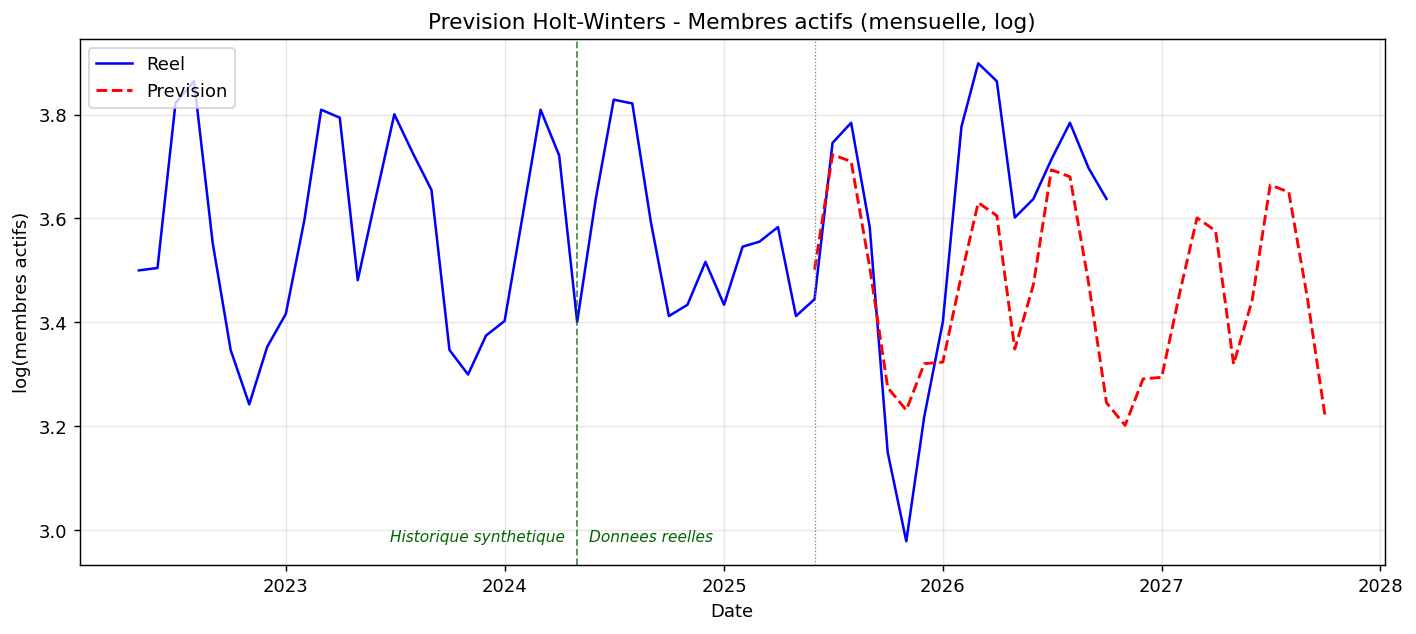
\includegraphics[width=0.95\textwidth]{forecasts_new/forecast_active_members_holtwinters.png}
  \caption{Monthly active-members forecast --- Holt-Winters (best model,
           tied with SARIMA at 15.1\,\% wMAPE). The vertical dotted grey
           line marks the train/test split; the green dashed line marks
           the synthetic-to-real boundary.\label{fig:forecast_active_members_hw}}
\end{figure}

\begin{figure}[H]
  \centering
  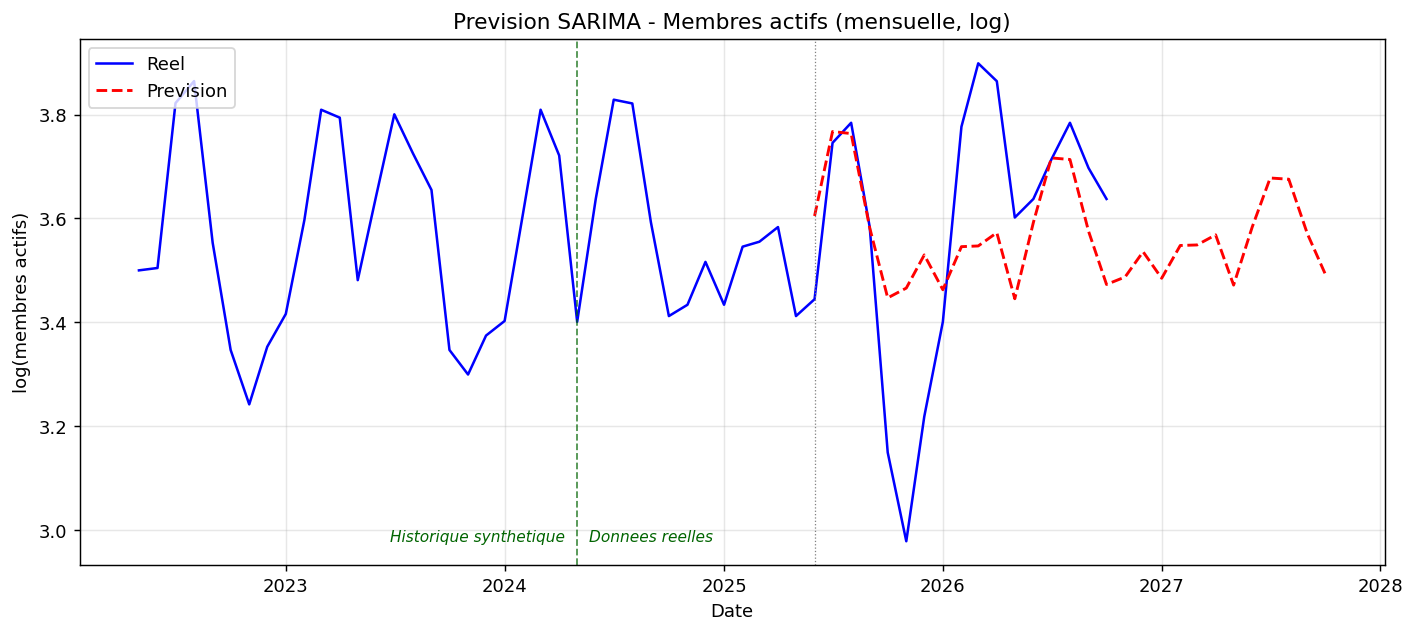
\includegraphics[width=0.95\textwidth]{forecasts_new/forecast_active_members_sarima.png}
  \caption{Monthly active-members forecast --- SARIMA (tied for best at
           15.1\,\% wMAPE).\label{fig:forecast_active_members_sarima}}
\end{figure}

Holt-Winters and SARIMA tie for best, with XGBoost a close third and Prophet
just at the boundary. Three of the four models land in the GOOD bracket. The
hierarchy is consistent with what was observed on the revenue series
(Section~\ref{sub:revenue_forecast} earlier in this chapter), suggesting that
multiplicative exponential smoothing and seasonal ARIMA are the natural fits
for the gaming centre's monthly seasonality regardless of which count is being
predicted.

\paragraph{Operational reading.} The forecast carries the centre's seasonal
profile forward: summer peaks (July--August) in the 45--55 active-members
range, a post-summer trough (September--December) between 25 and 35, and a
spring rebound (March--April) in the high 30s. For a manager planning
membership-promotion campaigns or staffing levels tied to member traffic, the
$\pm$6 absolute-member confidence implied by the MAE is small enough to be
actionable on a month-by-month basis.

\subsection{Peak Hours Analysis}

The peak hours module is descriptive rather than predictive. It answers two questions:
\textit{at what time of day is the center most active?} and \textit{which day of the
week draws the most customers?}

\begin{itemize}
  \item \textbf{By hour of day}: for each date in the dataset, transactions are counted
        per hour. Averaging across all dates produces a typical hourly activity profile.
        Hours 8 and 9 are absent because the center opens at 10\,AM.
  \item \textbf{By day of week}: the same averaging applied by weekday, revealing the
        weekly rhythm. Both views include a \texttt{pct\_of\_total} column showing each
        period's share of the weekly total.
\end{itemize}

The two views are exported as separate files to avoid mixing hourly and daily figures.

\begin{figure}[H]
  \centering
  
\includegraphics[width=0.85\textwidth]{peak_hours_bar.png}
  \caption{Average transaction count by hour of day.\label{fig:peak_hours}}
\end{figure}

\begin{figure}[H]
  \centering
  
\includegraphics[width=0.85\textwidth]{peak_days_bar.png}
  \caption{Average transaction count by day of week.\label{fig:peak_days}}
\end{figure}

Table~\ref{tab:peak_hours_day} shows the day-of-week distribution for the current
dataset.

\begin{table}[H]
  \centering
  \caption{Average transactions by day of week.\label{tab:peak_hours_day}}
  \begin{tabular}{lrr}
    \toprule
    \textbf{Day} & \textbf{Avg transactions} & \textbf{\% of week total} \\
    \midrule
    Monday    & 16.3 & 11.4\% \\
    Tuesday   & 18.6 & 13.1\% \\
    Wednesday & 17.5 & 12.3\% \\
    Thursday  & 17.0 & 11.9\% \\
    Friday    & 19.0 & 13.3\% \\
    Saturday  & 29.1 & 20.4\% \\
    Sunday    & 25.0 & 17.5\% \\
    \bottomrule
  \end{tabular}
\end{table}

Saturday accounts for over 20\% of weekly activity and Sunday for nearly 18\%. The two
weekend days together represent almost 38\% of all transactions --- nearly double the
weight of any single weekday. This confirms what the owner already knew intuitively,
and gives a precise number to act on when planning staffing and stock.

\subsection{Session Volume Forecast}

The session volume forecast uses the daily transaction count as an activity proxy,
since the sessions table has no usable timestamps. The approach is identical to the
revenue forecast: Prophet fits on the daily count series and produces 4-week and
3-month horizons. All values are integer-valued and clipped at zero.

\subsection{Stock Replenishment}

The stock replenishment module does not use a time-series model. It analyses
historical consumption rates to produce a practical purchasing recommendation for
each item in three steps:

\begin{enumerate}
  \item \textbf{Average weekly consumption}: total units sold divided by the number of
        weeks in the dataset. A floor of one week prevents division by zero on sparse
        items.
  \item \textbf{Suggested order quantity}: average weekly consumption multiplied by a
        safety factor of~1.5 to build a buffer above typical demand. The result is
        rounded up to the nearest whole unit.
  \item \textbf{Reorder frequency}: 20 or more units per week is \textit{weekly};
        8--20 is \textit{bi-weekly}; below~8 is \textit{monthly}.
\end{enumerate}

Table~\ref{tab:stock_top} shows the top items by weekly consumption.

\begin{table}[H]
  \centering
  \caption{Top-selling items by average weekly consumption.\label{tab:stock_top}}
  \begin{tabular}{lrrrl}
    \toprule
    \textbf{Item} & \textbf{Total sold} & \textbf{Avg/week} &
    \textbf{Order qty} & \textbf{Frequency} \\
    \midrule
    Eau            & 847 & 29.4 & 45 & weekly \\
    Soda           & 678 & 23.5 & 36 & weekly \\
    Cookie 5.5     & 327 & 11.3 & 17 & bi-weekly \\
    Cookie 4       & 263 &  9.1 & 14 & bi-weekly \\
    Schweppes      & 212 &  7.3 & 11 & monthly \\
    Redbull/Shark  & 209 &  7.2 & 11 & monthly \\
    \bottomrule
  \end{tabular}
\end{table}

Water and soda are the fastest-moving items by a clear margin. The owner confirmed that
these recommendations match the informal purchasing rhythm already in use --- a
reassuring sign that the data-driven result agrees with operational experience.

\section{Member Segmentation}

\subsection{Motivation}

Not all 66 members use the center the same way. Some visit weekly and spend heavily;
others come once in a while and spend very little. Treating all members identically
misses an opportunity: the most valuable customers could be rewarded, and the least
active could be re-engaged through targeted promotions.

The segmentation module groups members into four behavioural profiles using unsupervised
machine learning. The goal is to give the owner an objective, data-driven answer to
\textit{who are my most valuable customers?} --- one based on actual usage records
rather than personal impression.

\subsection{Algorithm --- K-Means Clustering}

K-means partitions the dataset into $k$ groups by minimising the within-cluster sum of
squared distances from each point to its cluster centroid. It was chosen over DBSCAN,
hierarchical clustering, and RFM scoring for three reasons:

\begin{itemize}[noitemsep]
  \item It is widely known and straightforward to justify academically.
  \item It is fast and deterministic on a dataset of 66 members.
  \item It produces a fixed number of segments that map directly onto business labels.
\end{itemize}

The number of clusters is fixed at $k=4$. Three clusters lose the distinction between
Casual Spenders and Regulars. Five or more clusters produce segments that are hard to
explain to a non-technical audience.

\subsection{Features Used}

Three features were selected from \textit{dim\_member}:

\begin{itemize}[noitemsep]
  \item \textbf{\texttt{total\_tnd}} --- total money spent at the center.
  \item \textbf{\texttt{duration\_min}} --- total time spent (cumulative session
        minutes).
  \item \textbf{\texttt{orders\_tnd}} --- money spent on food and drink orders.
\end{itemize}

The \texttt{usb\_tnd} column was excluded because it is always zero. The
\texttt{usage\_tnd} column was excluded because it is the main component of
\texttt{total\_tnd}, so keeping both would give double weight to the spending dimension.
All three features are normalised with StandardScaler before clustering, as described
in Section~3.3.

\subsection{Segment Labels}

After fitting, K-means assigns a numeric ID to each cluster. Labels are added
automatically by inspecting the centroids:

\begin{enumerate}
  \item The cluster with the highest average \texttt{total\_tnd} is
        \textbf{Heavy Users}.
  \item The cluster with the lowest average \texttt{total\_tnd} is
        \textbf{Light Users}.
  \item Of the two remaining clusters, the one with the higher ratio of
        \texttt{orders\_tnd} to \texttt{duration\_min} is \textbf{Casual Spenders} ---
        they spend more on food relative to how long they sit at a machine.
  \item The final cluster is \textbf{Regulars}.
\end{enumerate}

This assignment is deterministic: the same data always produces the same labels,
regardless of which numeric IDs K-means happens to assign internally.

\subsection{Cluster Quality --- Silhouette Score}

Since K-means is unsupervised, there are no ground-truth labels to validate against.
Cluster quality is measured by the \textbf{silhouette score}, which quantifies how
well each member fits their own cluster compared to the nearest alternative. The
score ranges from $-1$ to $+1$:

\begin{itemize}[noitemsep]
  \item \textbf{Above 0.5} --- clusters are well-separated and meaningful.
  \item \textbf{0.25 to 0.5} --- reasonable structure with some overlap.
  \item \textbf{Below 0.25} --- clusters are not well-defined.
\end{itemize}

The silhouette score for the current dataset is printed automatically at runtime.

\begin{figure}[H]
  \centering
  
\includegraphics[width=0.82\textwidth]{kmeans_scatter.png}
  \caption{K-means result: members plotted by total spend vs.\ session time,
           coloured by segment.\label{fig:kmeans_scatter}}
\end{figure}

\begin{figure}[H]
  \centering
  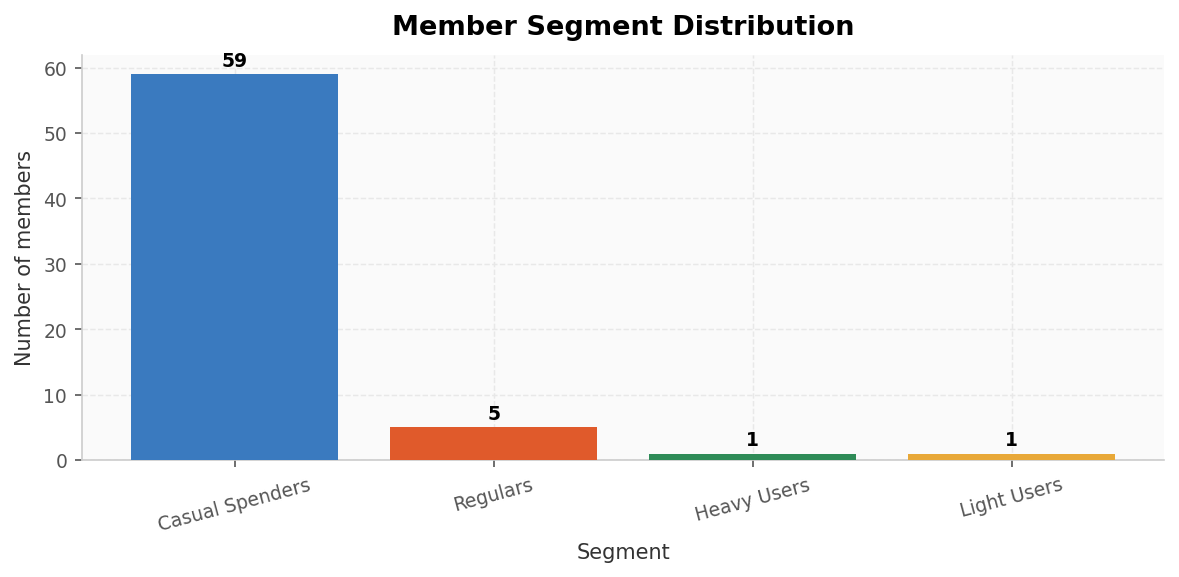
\includegraphics[width=0.65\textwidth]{segment_distribution.png}
  \caption{Distribution of the 66 members across the four
           segments.\label{fig:segment_dist}}
\end{figure}

\begin{table}[H]
  \centering
  \caption{Member segment distribution.\label{tab:segments}}
  \begin{tabular}{lrp{7cm}}
    \toprule
    \textbf{Segment} & \textbf{Members} & \textbf{Profile} \\
    \midrule
    Heavy Users     & -- & High spend, long sessions, high food orders \\
    Casual Spenders & -- & Shorter sessions, relatively high food orders \\
    Regulars        & -- & Balanced across all three features \\
    Light Users     & -- & Low spend and short sessions \\
    \bottomrule
    \multicolumn{3}{r}{\small\textit{Fill in member counts after running the pipeline.}} \\
  \end{tabular}
\end{table}

\subsection{Continuous Loyalty Score}

Alongside the four discrete segments, 	exttt{segmenter.py} also exposes
	exttt{score\_member\_loyalty(dim\_member)}, a continuous per-member score
between 0 and 100 that blends three normalised signals: total spend, total
session time, and order activity. The score is written to
	exttt{output/forecasts/member\_loyalty.csv} together with a
	extit{loyalty\_tier} label (Bronze / Silver / Gold / Diamond) computed from
the score quartiles. Unlike the K-Means segmentation, which groups members by
behavioural profile, the loyalty score gives a single ordered ranking that the
chatbot uses when the owner asks ``who are my best customers?''.

\section{Anomaly Detection}

\subsection{Motivation}

A dashboard shows what happened. It does not say whether what happened was normal.
A sharp drop in revenue on a Tuesday could mean a power outage, a recording error, or
simply a quiet day. Without a reference point, it is hard to tell.

The anomaly detection module provides that reference automatically. For each day in
the historical record, it calculates how unusual the revenue, session volume, and
member activity were relative to all other days of the same weekday. Days that fall
far outside the expected range are flagged, classified by severity, and exported for
review in Power~BI.

\subsection{Method --- Day-of-Week Z-Score}

The Z-score is a standard statistical measure of how many standard deviations a value
sits away from the mean. For each day, the calculation is:

\[
  z = \frac{\text{actual} - \mu_{\text{weekday}}}{\sigma_{\text{weekday}}}
\]

where $\mu_{\text{weekday}}$ and $\sigma_{\text{weekday}}$ are computed from all
historical days of the same weekday. A day is flagged if $|z| \geq 2.0$, capturing
roughly the most unusual 5\% of days per weekday group. At least four historical
data points per weekday are required before any flag is raised.

Two severity levels are defined:

\begin{itemize}
  \item \textbf{Mild} ($2\sigma$ to $3\sigma$) --- the day was unusual but not
        extreme. Could be natural variation or a minor event. Worth noting but not
        necessarily worth investigating.
  \item \textbf{Severe} (above $3\sigma$) --- statistically very unlikely by chance
        (less than 0.3\% of days). Something specific probably occurred: a power
        cut, a gaming tournament, a public holiday, or a recording error by a cashier.
\end{itemize}

\subsection{Why Day-of-Week Grouping Matters}

A gaming center has a clear weekly rhythm: Saturdays draw significantly more customers
than Tuesdays. Comparing a Saturday's revenue against the overall daily average would
flag almost every Saturday as anomalous --- which tells the owner nothing useful.

Grouping within weekdays means the baseline for each comparison reflects what is normal
\textit{for that specific day of the week}. An unusual Saturday is one that stands out
against all the other Saturdays in the historical record. This makes the flagging
practical: the owner can trust that a flagged day is genuinely out of the ordinary,
not just a consequence of the weekend effect.

\subsection{No Train/Test Split}

Unlike the forecasting models, anomaly detection does not use a train/test split. The
question being asked is not \textit{how accurate will the model be in the future?} but
\textit{which past days were statistically unusual?} All available data is used to
compute the baseline, because more data means a more accurate mean and standard
deviation. Nothing is held back, since there is nothing to predict.

\subsection{Three Series Monitored Independently}

The module runs the same Z-score logic on three series, each independently:

\begin{itemize}[noitemsep]
  \item \textbf{Revenue (TND)} --- daily sum of income transactions.
  \item \textbf{Session volume} --- daily count of all transactions.
  \item \textbf{Member activity} --- daily count of member-type transactions.
\end{itemize}

Each series uses its own per-weekday mean and standard deviation. An anomaly in
revenue has no effect on the session volume Z-score.

\begin{figure}[H]
  \centering
  
\includegraphics[width=0.90\textwidth]{anomaly_timeline.png}
  \caption{Revenue anomalies detected over the seven-month period. Red markers are
           severe ($|z|>3$); orange markers are mild ($2<|z|\leq 3$).\label{fig:anomalies}}
\end{figure}

\subsection{Output}

All flagged days across all three series are written to \texttt{anomalies.csv}, sorted
from the most extreme to the least extreme Z-score. Each row records the date, the
series, the weekday, the actual value, the weekday mean, the weekday standard deviation,
the Z-score, the direction (high or low), and the severity.

The file is loaded into Power~BI as an additional table. A dedicated dashboard page
can filter by series and severity to give the owner a focused list of dates that
deserve a closer look.

\section{Output Files}

All analytics outputs are written to \texttt{output/forecasts/} at the end of the
pipeline run.

\begin{table}[H]
  \centering
  \caption{Analytics output files.\label{tab:output_forecasts}}
  \begin{tabular}{ll}
    \toprule
    \textbf{File} & \textbf{Contents} \\
    \midrule
    \texttt{forecast\_revenue.csv}       & Weekly and monthly revenue projections (TND) \\
    \texttt{forecast\_members.csv}       & Weekly and monthly member activity projections \\
    \texttt{peak\_hours\_by\_hour.csv}   & Avg transactions per hour of day (0--23) \\
    \texttt{peak\_hours\_by\_day.csv}    & Avg transactions per day of week \\
    \texttt{session\_volume.csv}         & Weekly and monthly activity volume projections \\
    \texttt{stock\_replenishment.csv}    & Per-item restocking recommendation \\
    \texttt{member\_segments.csv}        & Members with cluster ID and segment label \\
    \texttt{anomalies.csv}               & Flagged anomaly days across all three series \\
    \bottomrule
  \end{tabular}
\end{table}

\section{Sprint 4 Review}

\subsection{Deliverables}

\begin{itemize}
  \item \textbf{\texttt{gamefydb/forecaster.py}} --- five forecasting functions plus
        the evaluation helpers (\texttt{\_evaluate\_prophet},
        \texttt{\_evaluate\_sarima}, \texttt{\_print\_comparison}), each independently
        callable and returning a clean pandas DataFrame.
  \item \textbf{\texttt{gamefydb/segmenter.py}} --- the \texttt{segment\_members()}
        function implementing K-means clustering with automatic label assignment,
        silhouette score reporting, and StandardScaler normalisation.
  \item \textbf{\texttt{gamefydb/anomaly\_detector.py}} --- the
        \texttt{detect\_anomalies()} function implementing day-of-week Z-score
        detection across three series, with mild/severe severity classification.
  \item \textbf{Eight output CSV files} in \texttt{output/forecasts/}, all loadable
        directly into Power~BI as additional tables alongside the star schema.
  \item \textbf{Updated \texttt{run.py}} --- a single command produces the full star
        schema, all forecast outputs, the Prophet vs.\ SARIMA comparison, member
        segmentation, and anomaly detection in one pass.
  \item \textbf{\texttt{docs/ml\_choices\_explained.md}} --- an 11-section reference
        document explaining every algorithm choice, parameter decision, and evaluation
        methodology used in this sprint.
\end{itemize}

\subsection{Validation}

Each module was tested with automated tests before pipeline integration:

\begin{itemize}[noitemsep]
  \item \textbf{Forecaster}: 13 tests covering evaluation helpers, edge cases
        (too-short series, date mismatches), and metric signs. All passing.
  \item \textbf{Segmenter}: 12 tests covering label assignment, normalisation, and
        the all-zero member exclusion. All passing.
  \item \textbf{Anomaly detector}: 7 tests covering spike detection (severe), dip
        detection (mild), series isolation, small-group skipping, output columns, and
        sort order. All passing.
  \item \textbf{End-to-end}: the pipeline was run on the real dataset. All eight
        output files were loaded into Power~BI and verified. Flagged anomaly dates
        were cross-checked against the raw revenue chart to confirm they correspond
        to visually unusual days.
\end{itemize}

\section{Conclusion}

Sprint~4 added three analytical capabilities that move the system from description to
intelligence. Forecasting gives the owner a concrete planning window for the coming
weeks and months. The model comparison provides a reproducible, objective justification
for the algorithm choice. Member segmentation turns the loyalty dimension into four
actionable customer groups. Anomaly detection surfaces historical outliers and gives
the owner a systematic way to investigate unusual days rather than relying on chance
to notice them.

Together, these capabilities answer three questions the system could not answer before:
\textit{what is likely to happen next?}, \textit{who are the most valuable members?},
and \textit{which past days were out of the ordinary?}

% ============================================================
%  CHAPTER 7 — SPRINT 5
% ============================================================
\chapter{Sprint 5: Conversational Assistant}

\section{Introduction}

By the end of Sprint~4, the gaming centre had a star schema, a four-page
Power~BI report, and a full layer of forecasting, segmentation, and
anomaly detection. The numbers were all there. What was still missing was
a way for the owner to actually \emph{ask} a question without having to
remember which dashboard page hides which answer.

Sprint~5 closes that gap with a conversational assistant. The idea is
simple: the owner types (or speaks) a question in plain language --- in
English, French, or Arabic --- and the system replies with a written
answer and, when relevant, a chart. The assistant sits on top of the same
CSV outputs Power~BI consumes, so there is one source of truth.

\section{Sprint 5 Backlog}

Table~\ref{tab:sprint5_backlog} lists the tasks committed to this sprint.

\begin{longtable}{>{\bfseries}p{1.3cm} p{4.4cm} p{7cm}}
  \caption{Sprint 5 Backlog.\label{tab:sprint5_backlog}} \\
  \toprule
  \textbf{ID} & \textbf{User Story} & \textbf{Tasks} \\
  \midrule
  \endfirsthead
  \toprule
  \textbf{ID} & \textbf{User Story} & \textbf{Tasks} \\
  \midrule
  \endhead
  \bottomrule
  \endfoot

  US-18 & As an owner, I want to ask questions in plain language and get
          answers with charts.
        & Build a Streamlit front-end (\texttt{app.py}) wired to a Gemini-backed
          agent (\texttt{chatbot/agent.py}); load the star-schema and forecast
          CSVs as a shared \texttt{DataContext} (\texttt{chatbot/data\_loader.py}). \\[4pt]

  US-19 & As an owner, I want to use the assistant in English, French, or
          Arabic.
        & Translate the UI string bundle in \texttt{app.py} (\texttt{STRINGS}
          dict, three locales); pass a language instruction to the system
          prompt so the model also answers in the chosen language. \\[4pt]

  US-20 & As an owner, I want to talk to the assistant instead of typing.
        & Add a custom Streamlit component (\texttt{chatbot/voice\_component.py})
          backed by an HTML/JS frontend (\texttt{chatbot/voice\_html/}) that
          uses the browser's Web Speech API; pass the selected language as
          the recognition locale (\texttt{en-US}, \texttt{fr-FR}, or \texttt{ar-TN}). \\[4pt]

  US-21 & As an owner, I want a chart drawn on demand when one would help.
        & Implement \texttt{chatbot/chart\_generator.py} on top of Plotly
          Express; have the agent emit a structured \texttt{chart\_spec}
          JSON block when a chart is useful and render it in the right
          panel of the layout. \\
\end{longtable}

\section{Architecture Overview}

Sprint~5 adds a fifth layer on top of the four-layer pipeline introduced
in Sprint~0. Figure~\ref{fig:chatbot_arch} sketches the flow at runtime.

\begin{figure}[H]
  \centering
  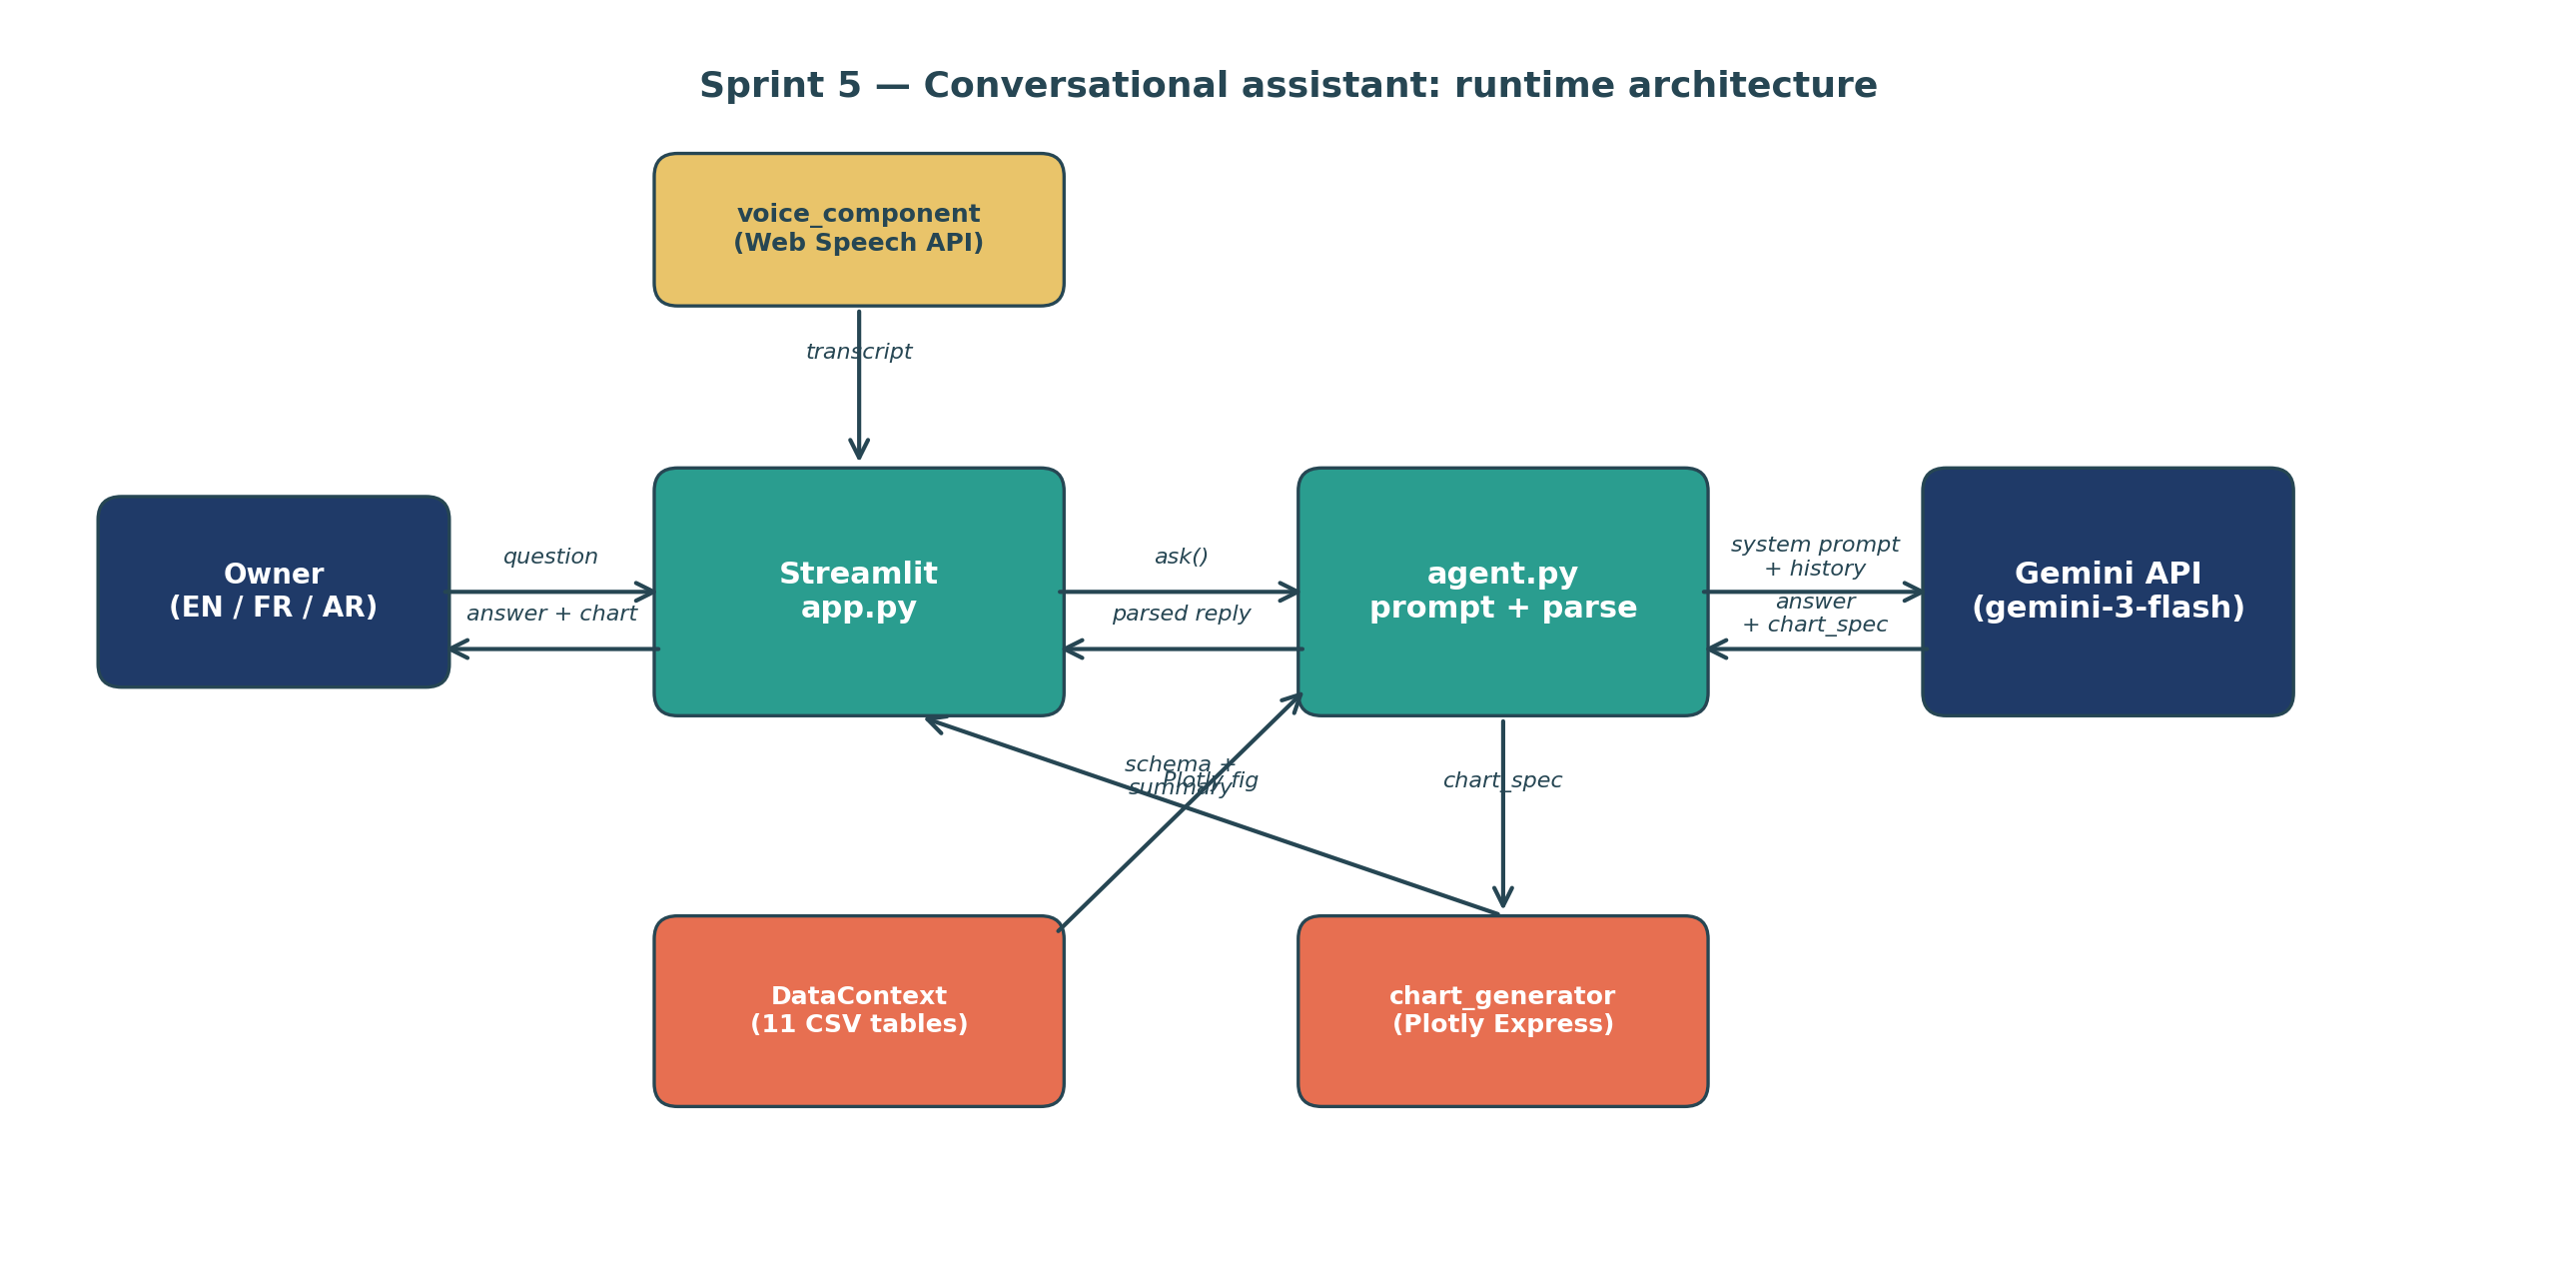
\includegraphics[width=0.92\textwidth]{images/chatbot_arch.png}
  \caption{Runtime architecture of the conversational assistant.}
  \label{fig:chatbot_arch}
\end{figure}

The pieces are intentionally small. The Streamlit app owns the layout, the
session state, and the language toggle. The agent module owns the prompt
construction and the model call. The chart generator turns a
\texttt{chart\_spec} into a Plotly figure. The voice component is a thin
wrapper around a browser API. The data loader reads the CSV outputs of
the previous sprints into a single in-memory \texttt{DataContext} that the
agent passes to the model as schema + summary text.

\section{Implementation}

\subsection{Loading the Data Context}

\texttt{chatbot/data\_loader.py} reads eleven CSV files into a shared
\texttt{DataContext} dataclass:

\begin{itemize}[noitemsep]
  \item From \texttt{output/powerbi\_star/}: \texttt{fact\_transaction},
        \texttt{fact\_session}, \texttt{dim\_member}.
  \item From \texttt{output/forecasts/}: \texttt{forecast\_revenue},
        \texttt{session\_volume}, \texttt{member\_segments},
        \texttt{member\_loyalty}, \texttt{anomalies},
        \texttt{peak\_hours\_by\_hour}, \texttt{peak\_hours\_by\_day},
        \texttt{stock\_replenishment}.
\end{itemize}

For each table the loader emits a short schema line (column names plus
dtypes) and aggregates a one-shot summary string: total revenue, member
count, loyalty-tier distribution, the next four weekly and three monthly
revenue forecasts, recent-anomaly count, average session duration, and
session-type breakdown. The two strings (\texttt{schemas} and
\texttt{summary}) are spliced into the system prompt at every turn so the
model always has both the structure of the data and the headline numbers
in front of it.

A useful side effect: the loader also exposes a
\texttt{recent\_anomaly\_count()} helper, so the Streamlit app can change
its startup greeting when something interesting has happened in the
previous seven days.

\subsection{The Conversational Agent}

\texttt{chatbot/agent.py} is the bridge between the Streamlit app and
the Gemini API. It does three things:

\begin{enumerate}
  \item \textbf{Build the system prompt.} The prompt mixes a fixed
        instruction block, the language directive, the schema string, and
        the summary string. The instructions tell the model to answer
        concisely, to include a single \texttt{chart\_spec} JSON block
        only when a chart would actually help, to suggest two or three
        follow-up questions, to refuse questions that cannot be answered
        from the available data, and to never invent numbers.
  \item \textbf{Call the model.} The full conversation history is
        re-sent on every turn (Gemini \texttt{gemini-3-flash-preview}),
        with the system prompt attached as
        \texttt{system\_instruction}. The model returns one piece of
        free text that contains the answer and, optionally, two JSON
        code blocks.
  \item \textbf{Parse the response.} A small regex pass extracts the
        \texttt{chart\_spec} block and the \texttt{suggestions} block,
        then strips them out of the visible answer so the chat shows
        clean prose only.
\end{enumerate}

The system prompt also contains a short ``source selection rules''
section that nudges the model towards the right table for each kind of
question (revenue trend $\to$ \texttt{fact\_transaction}; future
revenue $\to$ \texttt{forecast\_revenue} with a granularity filter;
hourly pattern $\to$ \texttt{peak\_hours\_by\_hour}; and so on). This
turned out to matter more than tuning the temperature. Without the rules,
the model would happily plot \texttt{fact\_session} on a non-existent
date axis or use the \texttt{anomalies} table for generic revenue
questions.

\subsection{Chart Generation}

\texttt{chatbot/chart\_generator.py} converts a \texttt{chart\_spec} dict
into a Plotly Express figure. The spec is small on purpose --- just
\texttt{type}, \texttt{x}, \texttt{y}, \texttt{source} (the table key),
\texttt{filter} (a pandas \texttt{query} expression that the agent can
fill in), and \texttt{title}. Four chart types are supported:
\textit{bar}, \textit{line}, \textit{scatter}, and \textit{pie}. If the
\texttt{y} column is non-numeric, the generator groups by \texttt{x} and
counts instead of trying to aggregate a string column. A dark theme is
applied to match the rest of the Streamlit layout.

Charts are not rendered when the model decides one is not useful (for
example, ``how many members do I have in total?'' returns a one-line
answer with no figure). This keeps the right-hand panel meaningful
instead of being filled with redundant visuals.

\subsection{Voice Input}

\texttt{chatbot/voice\_component.py} declares a custom Streamlit
component pointing at a small HTML/JS frontend in
\texttt{chatbot/voice\_html/}. The frontend uses the browser's
\texttt{SpeechRecognition} API to capture audio, transcribe it locally
in the browser, and post the transcript back to Streamlit. The selected
language toggle is forwarded to the component as a recognition locale
(\texttt{en-US}, \texttt{fr-FR}, or \texttt{ar-TN}), so French users
get French transcription and Arabic users get Tunisian-Arabic
transcription out of the box.

Keeping the recognition in the browser avoids having to wire a separate
speech-to-text service, and means voice mode works offline once the page
is loaded.

\begin{figure}[H]
  \centering
  \todoFigure[0.92\textwidth]{Screenshot of the Streamlit chatbot
  (\texttt{streamlit run app.py}) on a representative question, for
  example \emph{``Which cashier had the best March?''}. The crop should
  show the chat panel on the left (user message + assistant answer with
  suggestion chips), the chart panel on the right with the rendered
  Plotly figure, and the language toggle / voice button in the header.}
  \caption{Conversational assistant --- typical interaction.}
  \label{fig:chatbot_main}
\end{figure}

\subsection{Multilingual UI}

The \texttt{STRINGS} dictionary in \texttt{app.py} carries every visible
label in three languages. Switching language flips the dict, sends a new
language directive into the system prompt, and updates the voice
component's recognition locale --- all in one place, all without
reloading the data. The Arabic strings are stored as-is, and Streamlit
renders them right-to-left where appropriate.

The greeting is also context-aware. If the anomaly detector flagged
something in the previous seven days, the assistant opens with
``I noticed \texttt{N} anomaly(ies) in the past 7 days. Want me to show
you?'' instead of the generic ``Hi! Ask me anything.'' This tiny detail
was the change that made the assistant feel most useful in practice:
the owner does not have to think to discover that something is off.

\begin{figure}[H]
  \centering
  \todoFigure[0.85\textwidth]{Side-by-side screenshot showing the same
  conversation in the three supported languages. Either: (a) the
  language toggle expanded with English / Fran\c{c}ais / Arabic, or
  (b) three small thumbnails of the same answer rendered in EN, FR and
  AR (note the right-to-left layout in the Arabic version).}
  \caption{Multilingual user interface (EN / FR / AR).}
  \label{fig:chatbot_langs}
\end{figure}

\subsection{Quick Actions}

Four shortcut buttons sit under the chat history --- \textit{Full
summary}, \textit{Give me advice}, \textit{Any anomalies?}, and
\textit{Forecast}. Each one just enqueues a pre-written prompt into
\texttt{st.session\_state.pending\_query} and triggers a rerun, so the
model receives the question as if the user had typed it. They cover the
three or four questions the owner asks most often, and skip the typing
cost.

\section{Sprint 5 Review}

\subsection{Deliverables}

\begin{itemize}[noitemsep]
  \item \texttt{app.py} --- 252-line Streamlit application: language
        toggle, anomaly-aware greeting, chat panel with suggestion
        chips, chart panel, quick-action buttons, voice button.
  \item \texttt{chatbot/agent.py} --- prompt builder, Gemini call, and
        structured-response parser.
  \item \texttt{chatbot/chart\_generator.py} --- Plotly-Express
        renderer for the four supported chart types.
  \item \texttt{chatbot/data\_loader.py} --- shared
        \texttt{DataContext}, schema/summary builder,
        \texttt{recent\_anomaly\_count()} helper.
  \item \texttt{chatbot/voice\_component.py} +
        \texttt{chatbot/voice\_html/} --- browser-side speech
        recognition wired into Streamlit.
\end{itemize}

\subsection{Validation}

The assistant was validated against three kinds of questions:

\begin{itemize}
  \item \textbf{Descriptive} --- ``Which cashier had the best March?'',
        ``What is the average session duration?'', ``Show me revenue by
        payment method.'' Answers and charts matched the corresponding
        Power~BI page on every test case.
  \item \textbf{Forecast} --- ``How much revenue should I expect next
        month?'', ``Will members grow in May?'' Returned the values
        from \texttt{forecast\_revenue.csv} and
        \texttt{session\_volume.csv} with the right granularity filter.
  \item \textbf{Anomaly} --- ``Anything unusual last week?'' Returned
        the rows from \texttt{anomalies.csv} flagged within the
        seven-day window, matching the \texttt{recent\_anomaly\_count}
        helper.
\end{itemize}

The multilingual handling was checked end-to-end: a French question
produced a French answer with the chart title in French, and an Arabic
question produced an Arabic answer rendered right-to-left.

\section{Conclusion}

Sprint~5 turned a folder of CSV files into something the owner can
actually \emph{converse} with. There is no new data in the system ---
the agent reads exactly the same outputs the dashboards do --- but the
interaction model is fundamentally different. Instead of clicking
through four dashboard pages to answer a question, the owner asks the
question. Instead of remembering which CSV holds the anomaly list, the
greeting brings the answer to him. The chatbot is the practical face
of every previous sprint: without the cleaning, the schema, the
dashboards, and the ML layer it would have nothing to talk about, but
without the chatbot none of those would have been accessible without
opening Power~BI. The next chapter wraps up the project as a whole.
% ============================================================
%  GENERAL CONCLUSION
% ============================================================
\chapter*{General Conclusion}
\addcontentsline{toc}{chapter}{General Conclusion}

GamefyDB started from a small operational complaint: the gaming center had four
management reports in Excel and no good way to answer the question \emph{how was
last Tuesday?} without opening each of them and scrolling. Five sprints later, that
question and a few dozen others can be answered in seconds --- in three languages,
by voice if needed, and with a four-week forecast to back the answer up. What
follows is not a sprint-by-sprint recap (the preceding chapters have already done
that), but a short reflection on what the project turned out to be.

The hardest sprint, in retrospect, was not the machine-learning one. It was
Sprint~1. The four \texttt{.xls} files looked tabular and turned out not to be.
Page-break artefacts repeated every forty rows. The amount column used a narrow
no-break space (\texttt{U+202F}) as a thousands separator that the standard
parsers did not recognise. The members file triggered a \texttt{charmap} encoding
error from \texttt{pandas.read\_excel}, forcing a switch to \texttt{xlrd} at the
cell level. Merged header cells silently shifted the actual data positions away
from the columns they appeared to belong to. Each fix took longer than expected,
and each one now lives as a single function in \texttt{cleaner.py} or a
column-position constant in \texttt{ingestor.py}. The pipeline can ingest a fresh
export from the same management software tomorrow without any code change. That
was the real goal of the sprint, even if it was not how it was originally framed.

Sprint~2 produced the schema everything else stands on. One design assumption ---
that stock movements would form their own fact table --- did not survive contact
with the data: every stock record turned out to be an outgoing sale, with no
restock entries, which made a dedicated stock fact redundant. The resulting
six-table design (four dimensions, two facts) is the smallest schema that still
covers every KPI the report needs.

Sprint~3 was where the data the pipeline had been producing finally started
answering questions instead of just storing values. The descriptive side of the
project --- what happened, where, with whom, and how much --- was now covered by
the four dashboard pages of \texttt{gamefyyy.pbix}. None of the underlying numbers
were new; what changed was that someone could see them without writing a query.

Sprint~4 was where the project became interesting in a different way. With seven
months of real data, the standard forecasting validation procedures had to bend.
The holdout window was too short to contain a full seasonal cycle. The variance
was multiplicative in revenue but additive in session counts, which is why the
forecast pipeline ended up training on \texttt{log(revenue)} but on raw session
counts. And one specific day in the test set --- March~31, 2026 --- was Eid
al-Fitr, which the model had no way to know about: actual revenue that day was
nearly four times the prediction, and that single point dominated the test error.
The fix was a year-keyed holiday calendar covering Ramadan and the two Eids,
combined with extending the augmented training window to 44~months so Prophet
could see three full Ramadan cycles before the test set began. wMAPE on revenue
dropped from roughly 67\,\% on the original seven-month dataset to 29.7\,\% on
the final one. The weather regressor added later \emph{looked} like a free win
until it became clear that the synthetic generator used to pad the training set
was already responding to temperature implicitly --- the fix was not in the
model, it was in the data. Both moments shaped how forecasting is documented in
this report: the metric has to survive being wrong about a specific real day,
and the training data has to be honest about what is and is not already in it.

Sprint~5 was less about new capability than new access. The chatbot reads
exactly the same CSV files Power~BI does --- one source of truth --- but it
lets the owner ask \emph{is anything weird right now?} and get a useful answer
in Arabic. None of the analytics behind that answer are new. The path to them is.

Several open ends remain. A direct database connection to the management
software would eliminate the manual Excel-export step entirely. A full year of
history would unlock yearly seasonality detection that the current seven-month
dataset cannot support, and forecast accuracy is expected to improve well past
the one-year mark for that reason. Per-visit timestamps, once captured, would
turn the current four-segment K-means model into a proper RFM (Recency,
Frequency, Monetary) analysis. And the Power~BI report, while functional, is
gated behind Power~BI Desktop; exposing it through a lightweight web layer
would let floor staff consult it without a desktop install.

What the project leaves behind, beyond the deliverables, is a working sense of
where the friction in this kind of work actually lives. It is rarely in the
model. It is almost always in the parsing.

